
% YAML-metadata for possible future autogenerator
% ---
% language: finnish
% title_fi: Ajoneuvotietokoneen päivitysmahdollisuudet hakkuukoneessa
% title_en: Possibilities to upgrade Sunit Nero -embedded computer in Valmet 901 II -Harvester
% subtitle: Sunit Nero / Valmet 901 II
% author: Tomi Haapaniemi
% instructors_fi: Keijo Länsikunnas, Lehtori
% instructors_en: Keijo Länsikunnas, Lecturer
% keywords_fi: Hakkuukone, ajoneuvotietokone
% keywords_en: harvester, in-vehicle computer
% ---

%\begin{document}


%----------------------------------------------------------------------------------------
%    Tiivistelmä
%----------------------------------------------------------------------------------------

\thispagestyle{tiivis}
\begin{tabular}{ | p{4,7cm} | p{10,3cm} |}
  \hline
  Tekijä (t)\newline
  Otsikko \newline\newline

  Sivumäärä \newline
  Aika
  &
  \makeatletter
  \@author\newline
  \tiivistelmaotsikko\newline\newline
  \makeatother
  \pageref*{LastPage} sivua + \total{chapter} liitettä\newline %! if no appendices, risk to count total of chapter :D
  \pvm
  \\ \hline
  Tutkinto & \tutkinto
  \\ \hline
  Koulutusohjelma & \kohjelma
  \\ \hline
  Suuntautumisvaihtoehto & \suuntautumis
  \\ \hline
  Ohjaaja(t) & \ohjaajat
  \\ \hline
  \multicolumn{2}{|p{15cm}|}{\begin{singlespacing}\vspace{-22pt}
  %Tämä on tiivistelmän ensimmäinen kappale. Tiivistelmän kappaleet loppuvat komentoon newline, jotta saadaan yksi tyhjä rivi aikaiseksi. \newline
  Tämän insinöörityön tarkoituksena on selvittää 17 vuotta vanhan Valmet 901 II- hakkuukoneen ajoneuvotietokoneen korvausmahdollisuudet. Työ tehtiin yksityiselle yrittäjälle. Loppukäyttäjän (hakkuukoneen kuljettajan) toiveesta korvaus tulisi toteuttaa siten, että korvaavassa ajoneuvotietokoneessa toimisivat alkuperäisessä ajoneuvotietokoneessa käytetyt ohjelmistot. Työn tarkoituksena on tuottaa lisää tietoa käytössä olevan hakkuukoneen käyttöiän ennusteesta koneen tietotekniikan osalta. Tavoitteena oli saada hakkuukoneeseen toimintakuntoinen, fyysisiltä ulkomitoiltaan yhteensopiva ajoneuvotietokone alkuperäisen tilalle. Koska alkuperäinen järjestelmä osoittautuikin vielä korjauskelpoiseksi ja korvaavan järjestelmän tuottamisen arvioitiin vievän liikaa aikaa, päädyttiin insinöörityö rajaamaan selvitykseksi järkevän budjetin ja aikataulun rajoissa olevista päivitysmahdollisuuksista.\newline

  Haasteita työlle asetti hakkuukoneen sijainti metsässä 30 km Oriveden keskustasta, jonne on matkaa kotoani Kirkkonummelta noin 200 km. Prosessin aikana käytiin alkuperäisen ajoneuvotietokoneen huoltojen yhteydessä hakkuukoneen luona yhteensä kolme kertaa. Lisäksi laitetta ja sen osia huollettiin etätyönä yrittäjän lähetettyä ne postitse, jolloin matka Orivedelle ei ollut välttämätön.\newline

  Työssä selviää, että hakkuukoneen järjestelmien kommunikointi ajoneuvotietokoneen kanssa tapahtuu standardin RS-232 -sarjaväylän kautta ja käytettävät ohjelmat on mahdollista saada toimimaan uudemmissa käyttöjärjestelmissä. Tämä mahdollistaa uudempien ajoneuvotietokoneiden tai fyysiseltä kestävyydeltään vastaavien tietokoneiden käytön hakkuukoneessa ilman muutoksia hakkuukoneen järjestelmiin. Vaatimuksina uudelle tietokoneelle on lähinnä tarvittava olosuhteiden kesto sekä tarvittavat liittimet. Hakkuukoneen järjestelmät vaativat kaksi sarjaporttiliitäntää, joilla kommunikointi hakkuukoneen ja ajoneuvotietokoneen välillä tapahtuu. Hakkuukoneen sähköjärjestelmä on 24V, mikä tulee ottaa huomioon tietokoneen sähkönsyöttöä pohdittaessa. \newline

  Parhaana vaihtoehtona pidän tällä hetkellä ajoneuvotietokoneen korvaamista Panasonic Toughbook CF-19 tietokoneella. Myös Raspberry Pi 2-pohjainen ratkaisu on harkitsemisen arvoinen.\newline


 % Tämä on tiivistlemän toinen kappale.
  \end{singlespacing}} \\[14cm] \hline
  Avainsanat & \avainsanat
  \\ \hline
\end{tabular}
\clearpage

%----------------------------------------------------------------------------------------
%	ABSTRACT
%----------------------------------------------------------------------------------------

\pagestyle{abstract}
\begin{tabular}{ | p{4,7cm} | p{10,3cm} |}
  \hline
  Author(s) \newline
  Title \newline\newline
  Number of Pages \newline
  Date
  &
  \makeatletter
  \@author \newline
  \@title \newline
  \pageref*{LastPage} pages + \total{chapter} appendices \newline %! if no appendices, risk to count total of chapter :D
  \IfLanguageName {finnish} {\foreignlanguage{english}{\longdate\@date}} {\@date}
  \makeatother
  \\ \hline
  Degree & \metropoliadegree
  \\ \hline
  Degree Programme & \metropoliadegreeprogramme
  \\ \hline
  Specialisation option & \metropoliaspecialisation
  \\ \hline
  Instructor(s) & \metropoliainstructors
  \\ \hline
  \multicolumn{2}{|p{15cm}|}{\begin{singlespacing}\vspace{-22pt}

The purpose of this thesis is to find out whether it is possible to replace the original computer in 17 y. old harvester with a newer computer so that there is no need to do any changes to the harvester's electronical systems. Therefore original communication protocols and controlling software must work in the new computer. User Experience of system with the new computer should be similar with the original computer.\newline

This thesis was done for a private entrepreneur and the results are intended to provide additional information about the life expectation of harvester from the viewpoint of computer systems. The original goal of the thesis was to produce a drop in -replacement computer for the original systems, but because the original system proved to be repairable and the time estimation for producing a durable replacement was too high it was decided to limit the thesis to be only a report about the possibility to upgrade the original system with reasonable budget and time.\newline

The location of the harvester, which was approx. 30 km to forest from the Orivesi city center set some challenges for the thesis. Distance to Orivesi is approx. 200 kilometres from my home at Kirkkonummi. Harvester was visited total of three times. All visits took place after maintenance of the harvester's original computer. In addition the entrepreneur sent some parts for maintenance by mail so that a visit to Orivesi wasn't necessary.\newline

Result of the thesis is that all required communication with harvester is through standard RS-232 serial bus. All required software was proven to work in newer operating systems which allows the possible new system to be selected from a broader range of availabe rugged computer models without any modifications to harvester's electronical systems. \newline

Requirements for a new computer are durability in existing conditions and availability of required connectors. The harvester's systems require two serial port connections for communication between harverter's systems and vehicle computer. The harvester's electrical system is 24V DC, which must be taken into account when selecting the computer's power supply.

In my opinion, currently the best option for the vehicle computer replacement is Panasonic Toughbook CF-19 laptop. Also, Raspberry Pi 2-based solution is worth considering.


  \end{singlespacing}} \\[14cm] \hline
  Keywords & \metropoliakeywords
  \\ \hline
\end{tabular}
\clearpage

%----------------------------------------------------------------------------------------
%	Acknowledgement ?
%----------------------------------------------------------------------------------------
%\chapter*{Acknowledgement}
%Thanks to my cat
%\clearpage

%----------------------------------------------------------------------------------------
%	TABLE OF CONTENTS
%----------------------------------------------------------------------------------------

\makeevenhead{plain}{}{}{}
\makeoddhead{plain}{}{}{}
\pagestyle{empty} %remove page number in toc (if longer than 2 pages)
\tableofcontents*
\pagestyle{empty} %remove page number in toc (if longer than 1 pages)
\clearpage
\pagestyle{plain}

%list of figure, tables comes here...


%----------------------------------------------------------------------------------------
%    Lyhenteet / Abbreviation
%----------------------------------------------------------------------------------------

\pagestyle{empty}
\setlength{\parskip}{1cm}
\IfLanguageName {finnish} {
  \chapter*{Lyhenteet}
  \cftaddtitleline{toc}{chapter}{Lyhenteet}{}
} {
  \chapter*{Abbreviation}
  \cftaddtitleline{toc}{chapter}{Abbreviation}{}
}
\begin{table}[h]
\setlength{\tabcolsep}{8pt}
\renewcommand{\arraystretch}{2}
\begin{tabular}{l p{12cm}}
x86 & Yleisnimitys Intelin 1987 julkaisemalle CISC-prosessorikäskykannalle. Työssä x86:lla viitataan myös 80386:ssa käytössä olleeseen ja myöhempiin 32-bittisiin versioihin kyseisestä käskykannasta.\\
PS/2 & Sarjaväyläinen, alunperin IBM PS/2 koneessa ollut liitäntäprotokolla, joka yleistyi PC-koneiden standardiliitännäksi näppäimistölle ja hiirelle ennen USB-protokollaa.\\
RS232 & Alunperin v. 1962 esitelty asynkroninen sarjaliitäntäprotokolla, joka oli ennen USB-liitännän yleistymistä yleisin PC-koneiden oheislaitteiden liitäntäväylä.\\
USB & Universal Serial BUS, vuonna 1996 esitelty sarjaväyläinen liitäntä oheislaitteiden liitäntään.\\
IDE/PATA & Integrated Drive Electronics (Parallel AT Attachments), kiintolevyjen ja optisten asemien liittämiseen tarkoitettu 16-bittinen rinnakkainen liitäntäväylä vuodelta 1986.\\
CAN & Controller Area Network, vikasietoinen, differentiaalinen kaksijohtoinen automaatioväylä, jossa liikenne lähetetään priorisoituina sanomina vuodelta 1986\\
Apteeraus & Puun rungon jako eri puutavaralajeiksi mitta- ja laatuvaatimukset huomioiden\\
GPS & Global Positioning System, Maapalloa kiertäviin satelliitteihin perustuva paikannusjärjestelmä\\
DPGS & Differential GPS, DGPS:ssä tarkennetaan sijaintitietoa käyttämällä apuna kiinteiden maa-asemien mittaamaa ja välittämää alueellista paikannusvirhettä.\\
Hypervisor & Järjestelmä tai ohjelmisto joka hallitsee ja suorittaa virtuaalikoneita.\\
%
%OMG & Oh my god\\
%WTF & What the F\\
%TL;DR & Too long, didn't read\\
\end{tabular}
\end{table}

\newpage

%page number always on top right; also for chapter "title" page
\pagestyle{plain}
\makeevenhead{plain}{}{}{\thepage}
\makeoddhead{plain}{}{}{\thepage}

\setcounter{page}{1} %page 1 should be Introduction
\ClearWallPaper
%----------------------------------------------------------------------------------------
%	CONTENT
%----------------------------------------------------------------------------------------

\chapter{Johdanto}

Tietokoneiden käyttöikä on varsinkin vaativissa kohteissa rajallinen. Kun järjestelmät vanhenevat, niin huollon tarve lisääntyy, mutta varaosien saatavuus vähenee. Viimein voi tulla eteen piste, jossa ainoa mahdollinen vaihtoehto on korvata vanha järjestelmä uudella. Tämä saattaa vaatia suuriakin muutostöitä myös järjestelmää käyttäviin laitteisiin ja usein on järkevämpää vaihtaa koko kohde kuin tehdä siihen suuria muutostöitä.

Insinöörityön kohteena on vuonna 1998 valmistetun hakkuukoneen ajoneuvotietokoneen päivitysmahdollisuuksien tutkiminen. Alkuperäisessä, myös vuodelta 1998 olevassa ajoneuvotietokoneessa on alkanut näkyä ikääntymisen merkkejä. Laitteen komponentit hajoavat yksitellen ja se ylikuumenee etenkin kesäisin siten, että käyttöaika on vain pari tuntia kerrallaan. Osien saatavuus näin vanhaan tietokoneeseen alkaa luonnollisesti olemaan hankalaa.

Insinöörityö pyrkii selvittämään hakkuukoneen ja ajoneuvotietokoneen väliset liitännät sekä ajoneuvotietokoneen ohjelmistot ja etsimään mahdolliset korvaavat ratkaisut. Tarkoituksena on, että loppukäyttäjän (hakkuukoneen kuljettajan) toiveesta korvaava järjestelmä vaatisi mahdollisimman vähän muutoksia hakkuukoneeseen sekä olisi hakkuukoneen kuljettajalle toiminnallisuudeltaan vastaava kuin alkuperäinen järjestelmä.

Haasteita työlle tuovat huollettavan hakkuukoneen sijainti yli 200 kilometrin päässä sekä alkuperäisten ohjelmien mahdollisesti asettamat vaatimukset. Lisäksi on huomioitava hakkuukoneen käyttöympäristö, joka asettaa ajoneuvotietokoneelle erityisiä vaatimuksia pölyn siedon, lämpötilan muutosten sekä tärinän keston suhteen. Lähtötilanteessa käytetyistä/alkuperäisestä järjestelmistä ei ollut lainkaan tietoja, eikä tiedetty miten ja mitä käyttöjärjestelmiä käyttäen järjestelmä on toteutettu.

\newpage

\chapter{Nykyinen järjestelmä}

\section{VALMET 901 II}

Hakkuukoneet eli motot (monitoimikoneet) ovat metsätraktoreita, joiden tehtävänä on hakkuun kaikki työvaiheet. Hakkuukoneet sisältävät tietokoneohjatut mittalaitteet, joilla puiden katkonta ja mittaus saadaan hoidettua tarkasti.

Työn kohteena oleva hakkuukone on nelipyöräinen Valmet 901 II vuosimallia 1998. Kone on otettu käyttöön joulukuussa 1998. Värityksenä on Valmetin vanhempi punamusta-väritys. Valmet 901 on Valmetin sen aikaisen malliston pienin hakkuukone, joka on tarkoitettu ensisijaisesti harvennushakkuisiin. Alkuperäinen hakkuupää on jälkikäteen vaihdettu toiseksi, jolloin myös apteeraukseen käytettävä ohjelmisto vaihtui. Hakkuukoneen alkuperäinen teleskooppipuomisto on vaihdettu liikeratapuomiksi.
\newline

\begin{figure}[H]
\centering
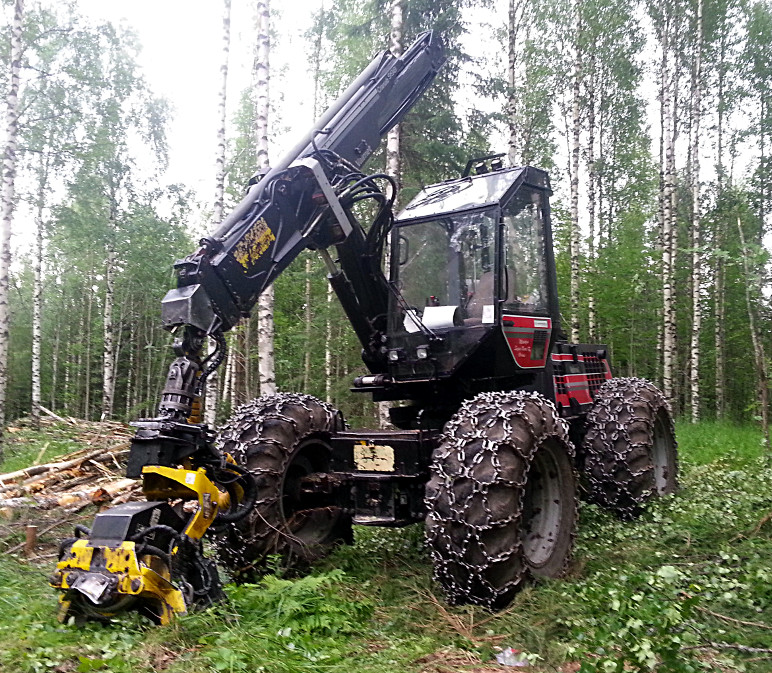
\includegraphics[width=0.700\textwidth]{moto_2.jpg}
\caption{Valmet 901 II}
\end{figure}

\section{Motomit-mittalaite}

Työn kohteena olevaan hakkuukoneeseen on jälkiasennettu Motomit-IT
-mittalaite, joka on korvannut hakkuukoneen alkuperäiset mittalaitteet
ja ohjelmiston. Motomit IT tukee StanForD-standardin mukaista
apteerausohjeiden tiedonsiirtoa. Motomit IT hoitaa sisäisen
kommunikaation CAN-väylää pitkin. Kommunikaatiossa alkuperäisen
ajoneuvotietokoneen kanssa käytetään RS232-väylää ja MotomitPC
-ohjelmistoa. (P. L. Oy 2008)
\newline

\begin{figure}[H]
\centering
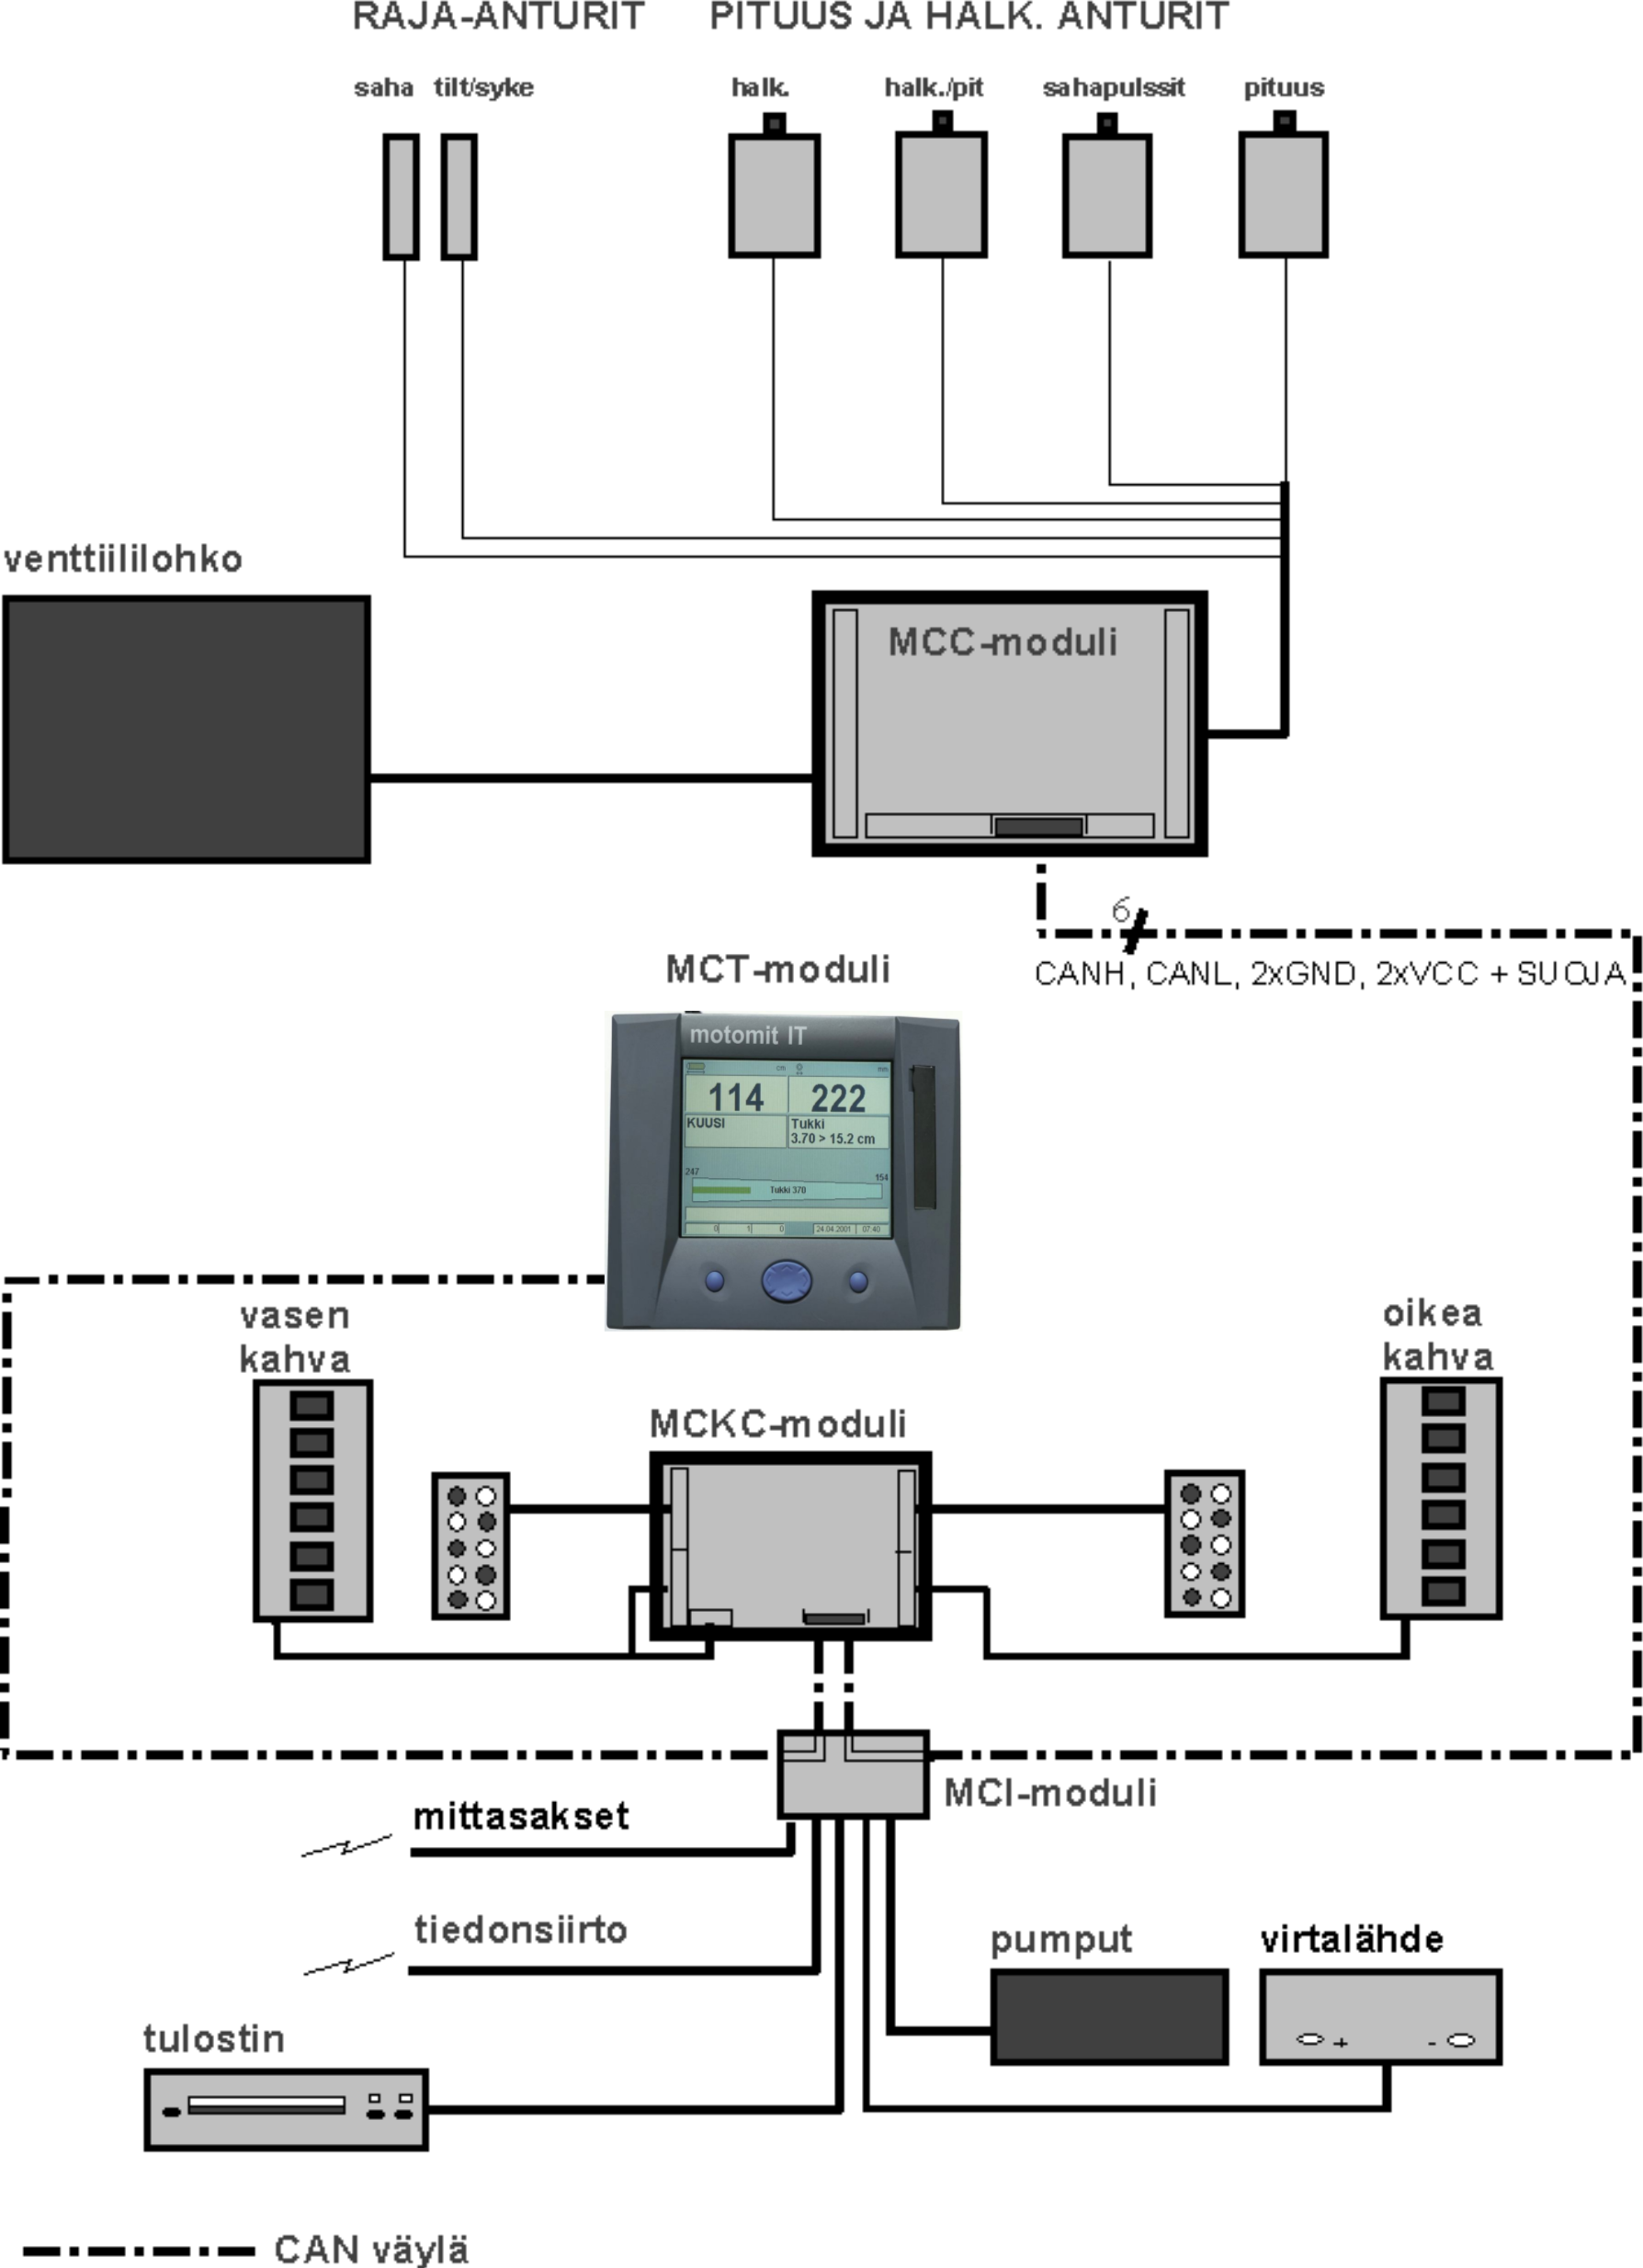
\includegraphics[width=0.800\textwidth]{motomit_kaavio.png}
\caption{Motomit IT:n moduulikaavio}
\end{figure}
\newpage

Motomit PC on Motomit IT:n Windows-pohjainen näyttö- ja hallintaohjelmisto Motomit IT-järjestelmälle. Motomit PC kommunikoi Motomit IT:n MCI-moduulin (Mitron CAN Interface) kanssa RS-232 -sarjaväylän avulla.
 \cite{motomit:esite}.
\newline
\begin{figure}[H]
\centering
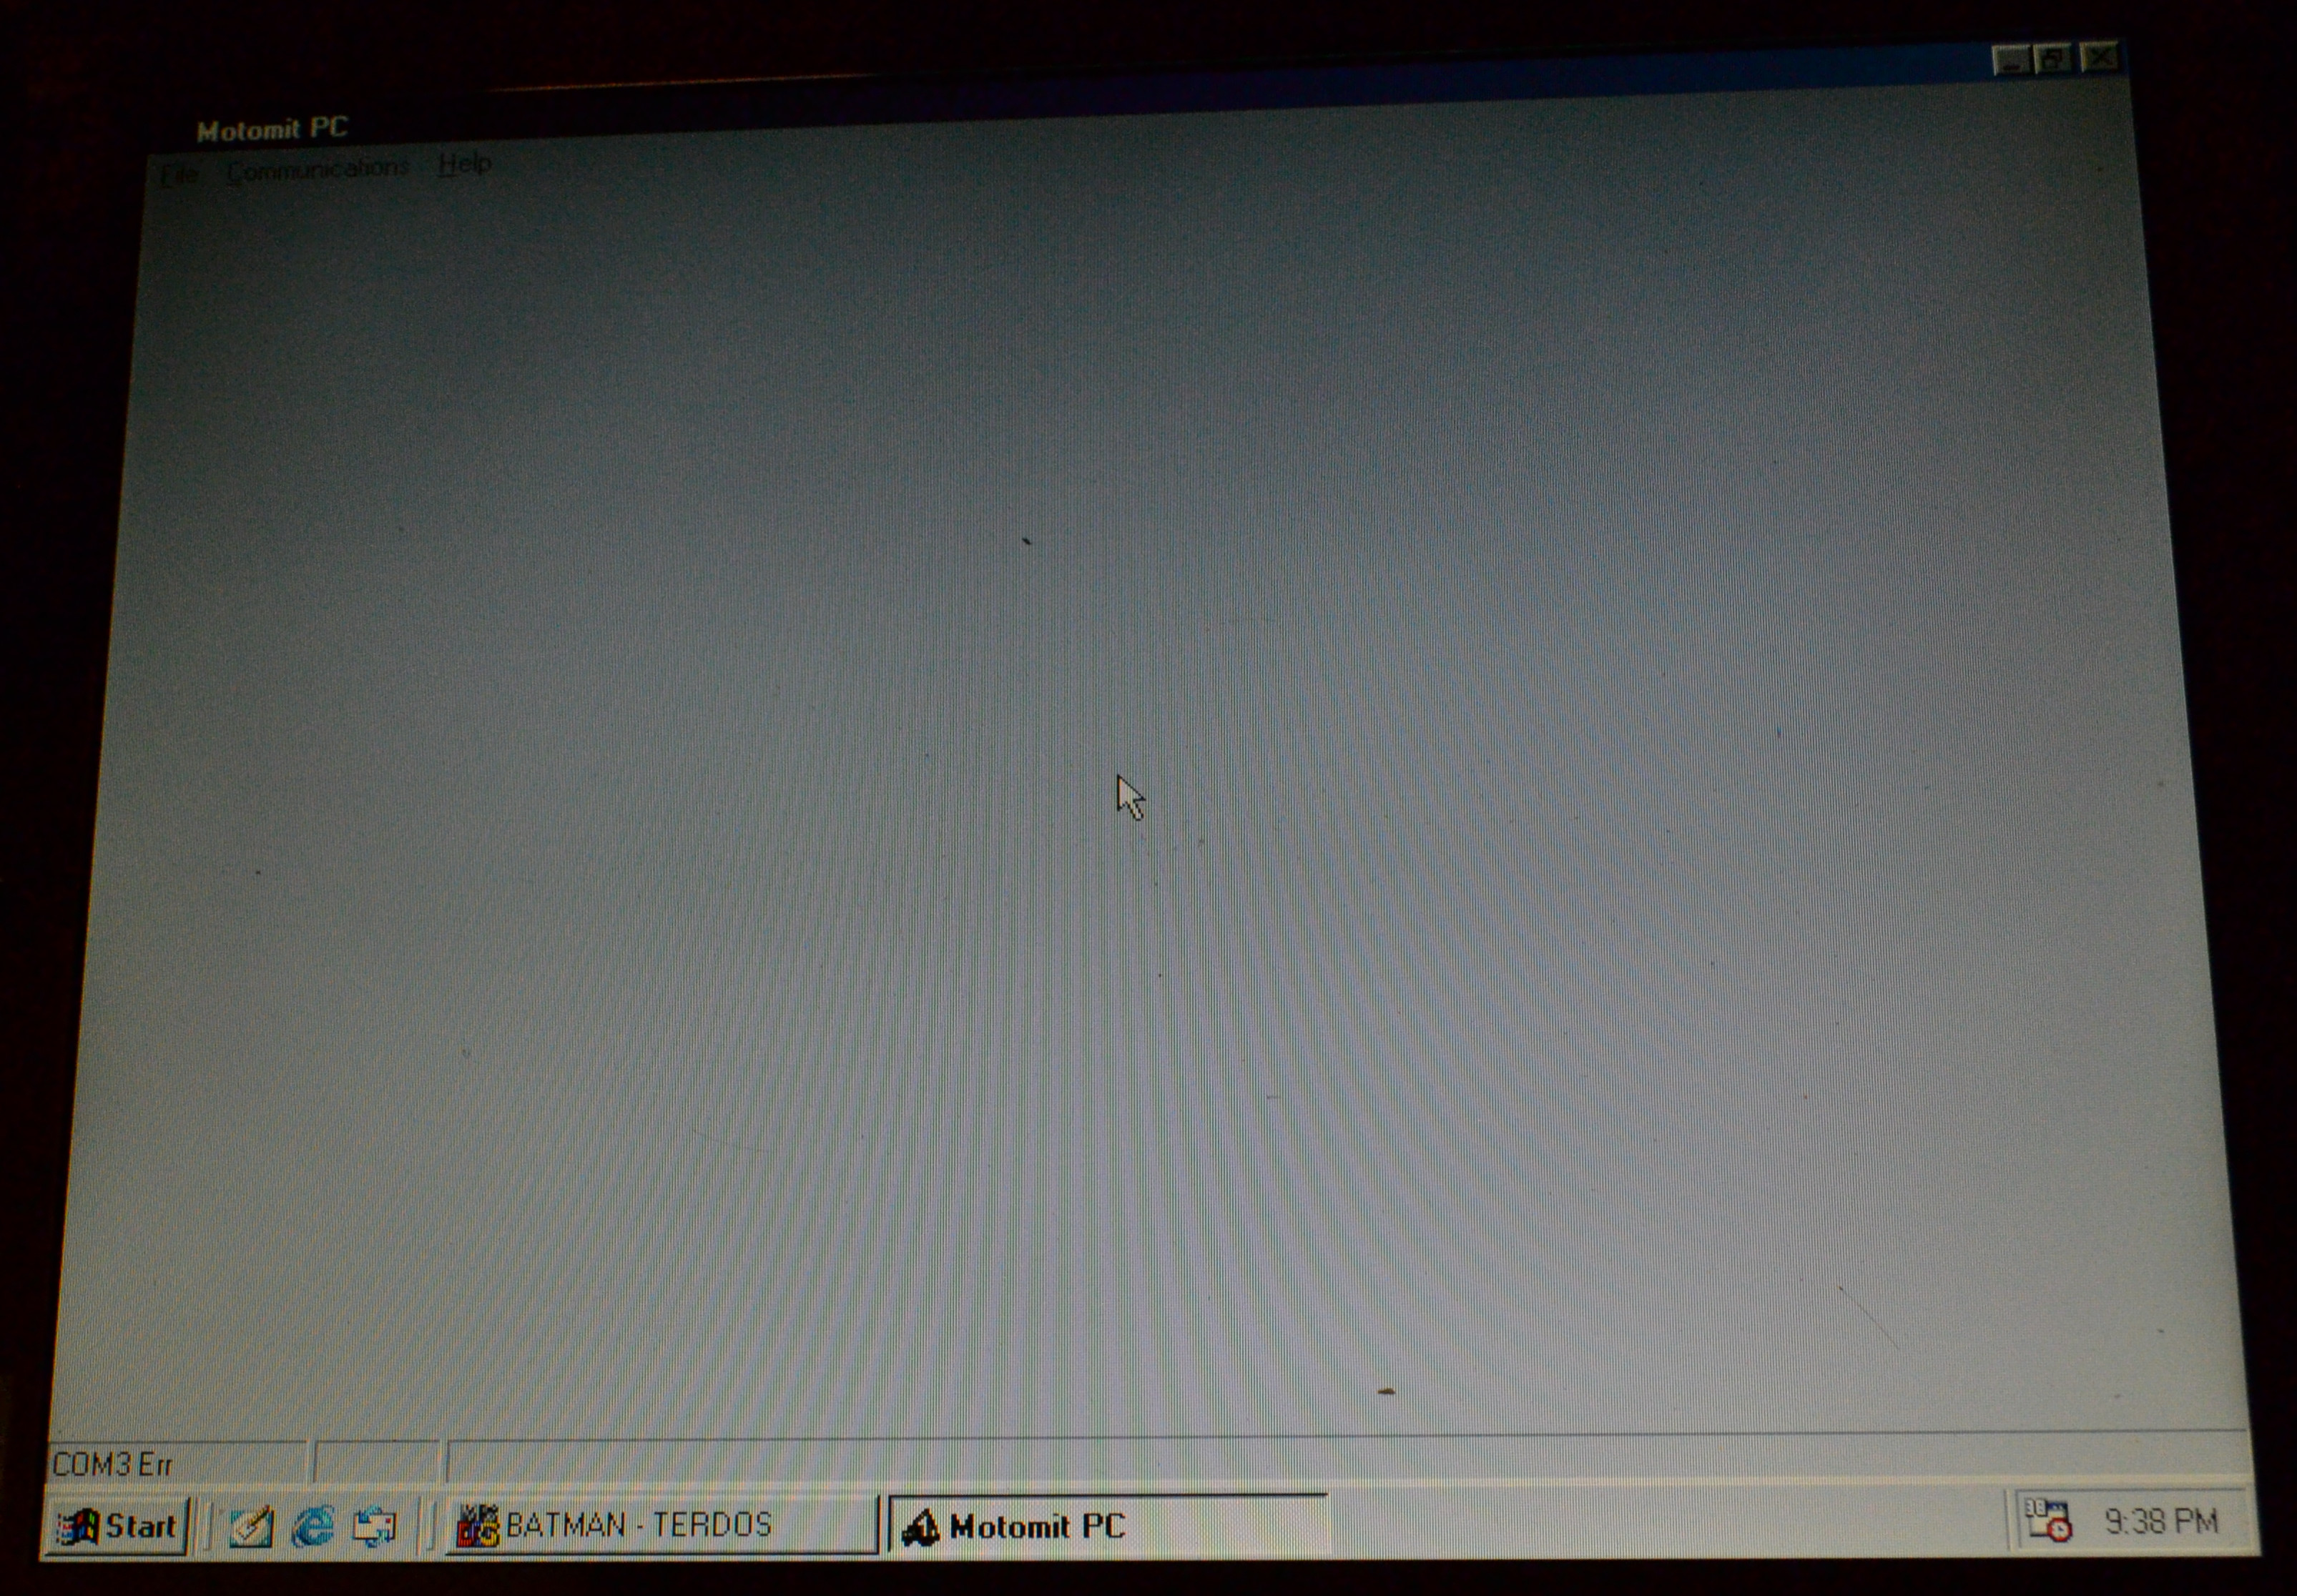
\includegraphics[width=1.00\hsize]{motomit_original.jpg}
\caption{Motomit PC Nero-ajoneuvopc:n ruudulla}
\end{figure}

\section{Ajoneuvo-PC Sunit Nero / Valmet Maxi}

Hakkuukoneessa käytetty tietokone on Sunitin valmistama Sunit Nero (myös nimellä Valmet MAXI)-ajoneuvotietokone. Nero on paketoitu näyttöineen ja keskusyksikköineen yhdeksi all-in-one -tyyliseksi iskunkestäväksi paketiksi. Vaikka kyseessä ei olekaan sama yksilö mikä on alunperin ollut kiinni kyseisessä hakkuukoneeessa, on se samanlainen kuin alkuperäinen ja samaa ikäluokkaa (noin 17 vuotta, vuodelta 1998). Tietokoneen mitat ovat 315 mm x 252 mm x 115 mm ja paino 4,2 kg. Virrankulutus Nerolla on n. 25W.

Nero täyttää CEN:n standardin EN55022 class A ja class B -vaatimukset ja Sunit vakuuttaa laitteen täyttävän EU:n direktiivien vaatimukset CE-merkinnällä. Neron kotelointi on tuuletusta lukuunottamaat IP54-luokkaa, joka tarkoittaa suojausta pölyltä, sekä suojausta vesiroiskeita vastaan. \cite{nero:manual}

\begin{figure}[H]
\centering
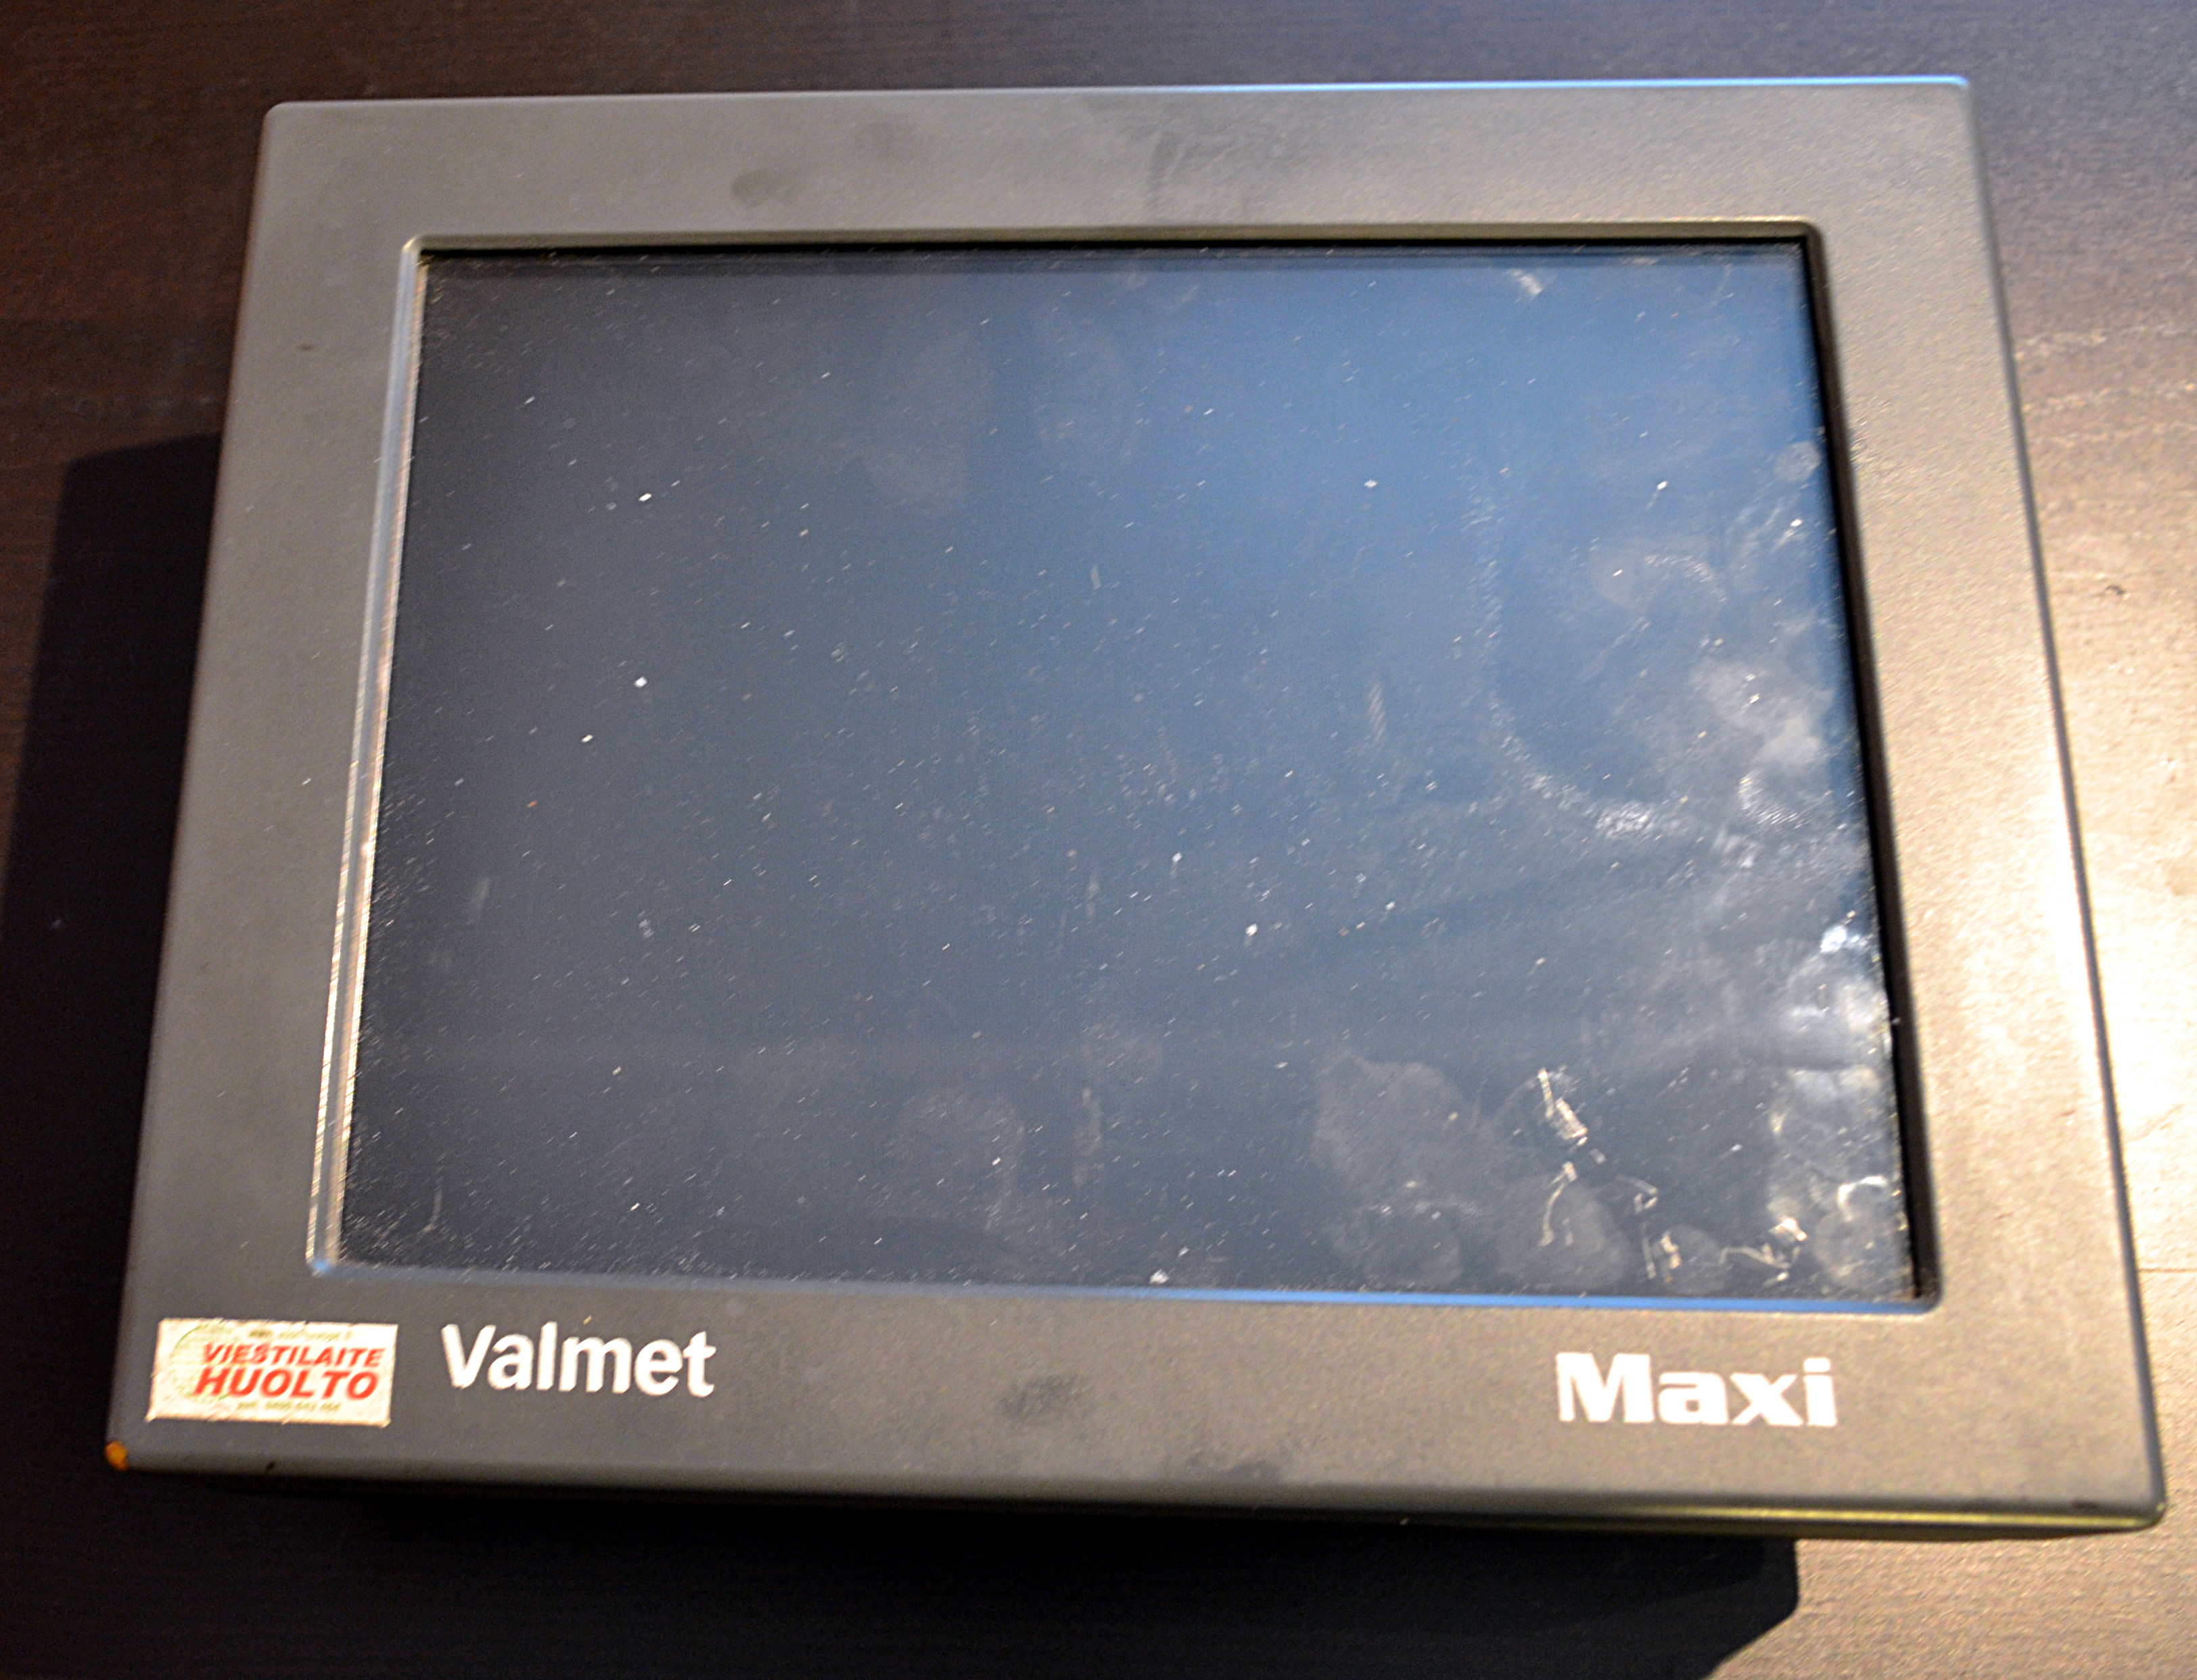
\includegraphics[width=1.000\hsize]{valmet_maxi.jpg}
\caption{Sunit Nero / Valmet Maxi}
\end{figure}

Sunit Nero osoittautui olemaan toteutettu PC-tekniikalla, sisältäen tavallisen x86-prosessorin ja Windows 98-käyttöjärjestelmän. Emolevyn northbridge-ohjaimena on SiS 5571-ohjain. Tässä Nero-yksilössä prosessorina on AMD:n 300 MHz Socket 7-kantainen K6-prosessori vuodelta 1998 (alkuperäinen prosessori on vaihdettu useita vuosia sitten tehdyn huollon yhteydessä toiseen), 64 Mb keskusmuistia. Tietokoneen kiintolevynä oli tutkintahetkellä Western Digitalin 120 Gb:n Scorpio Blue-kiintolevy, joka sekin on vaihdettu kyseiseen yksilöön useaan kertaan. Nero-tietokoneesta löytyy 3,5" levykseasema, sekä cd-asema. Näyttöpaneelissa on 12" LCD-paneeli 800x600 pikselin resoluutiolla. Kuvasuhde on 4:3. Lisäksi koneessa on NiMH-akku BIOSin asetusten säilyttämiseen. Tietokoneesta löytyy liitännät sekä 12V että 24V jännitteille.
\newline\newline

\begin{figure}[H]
\centering
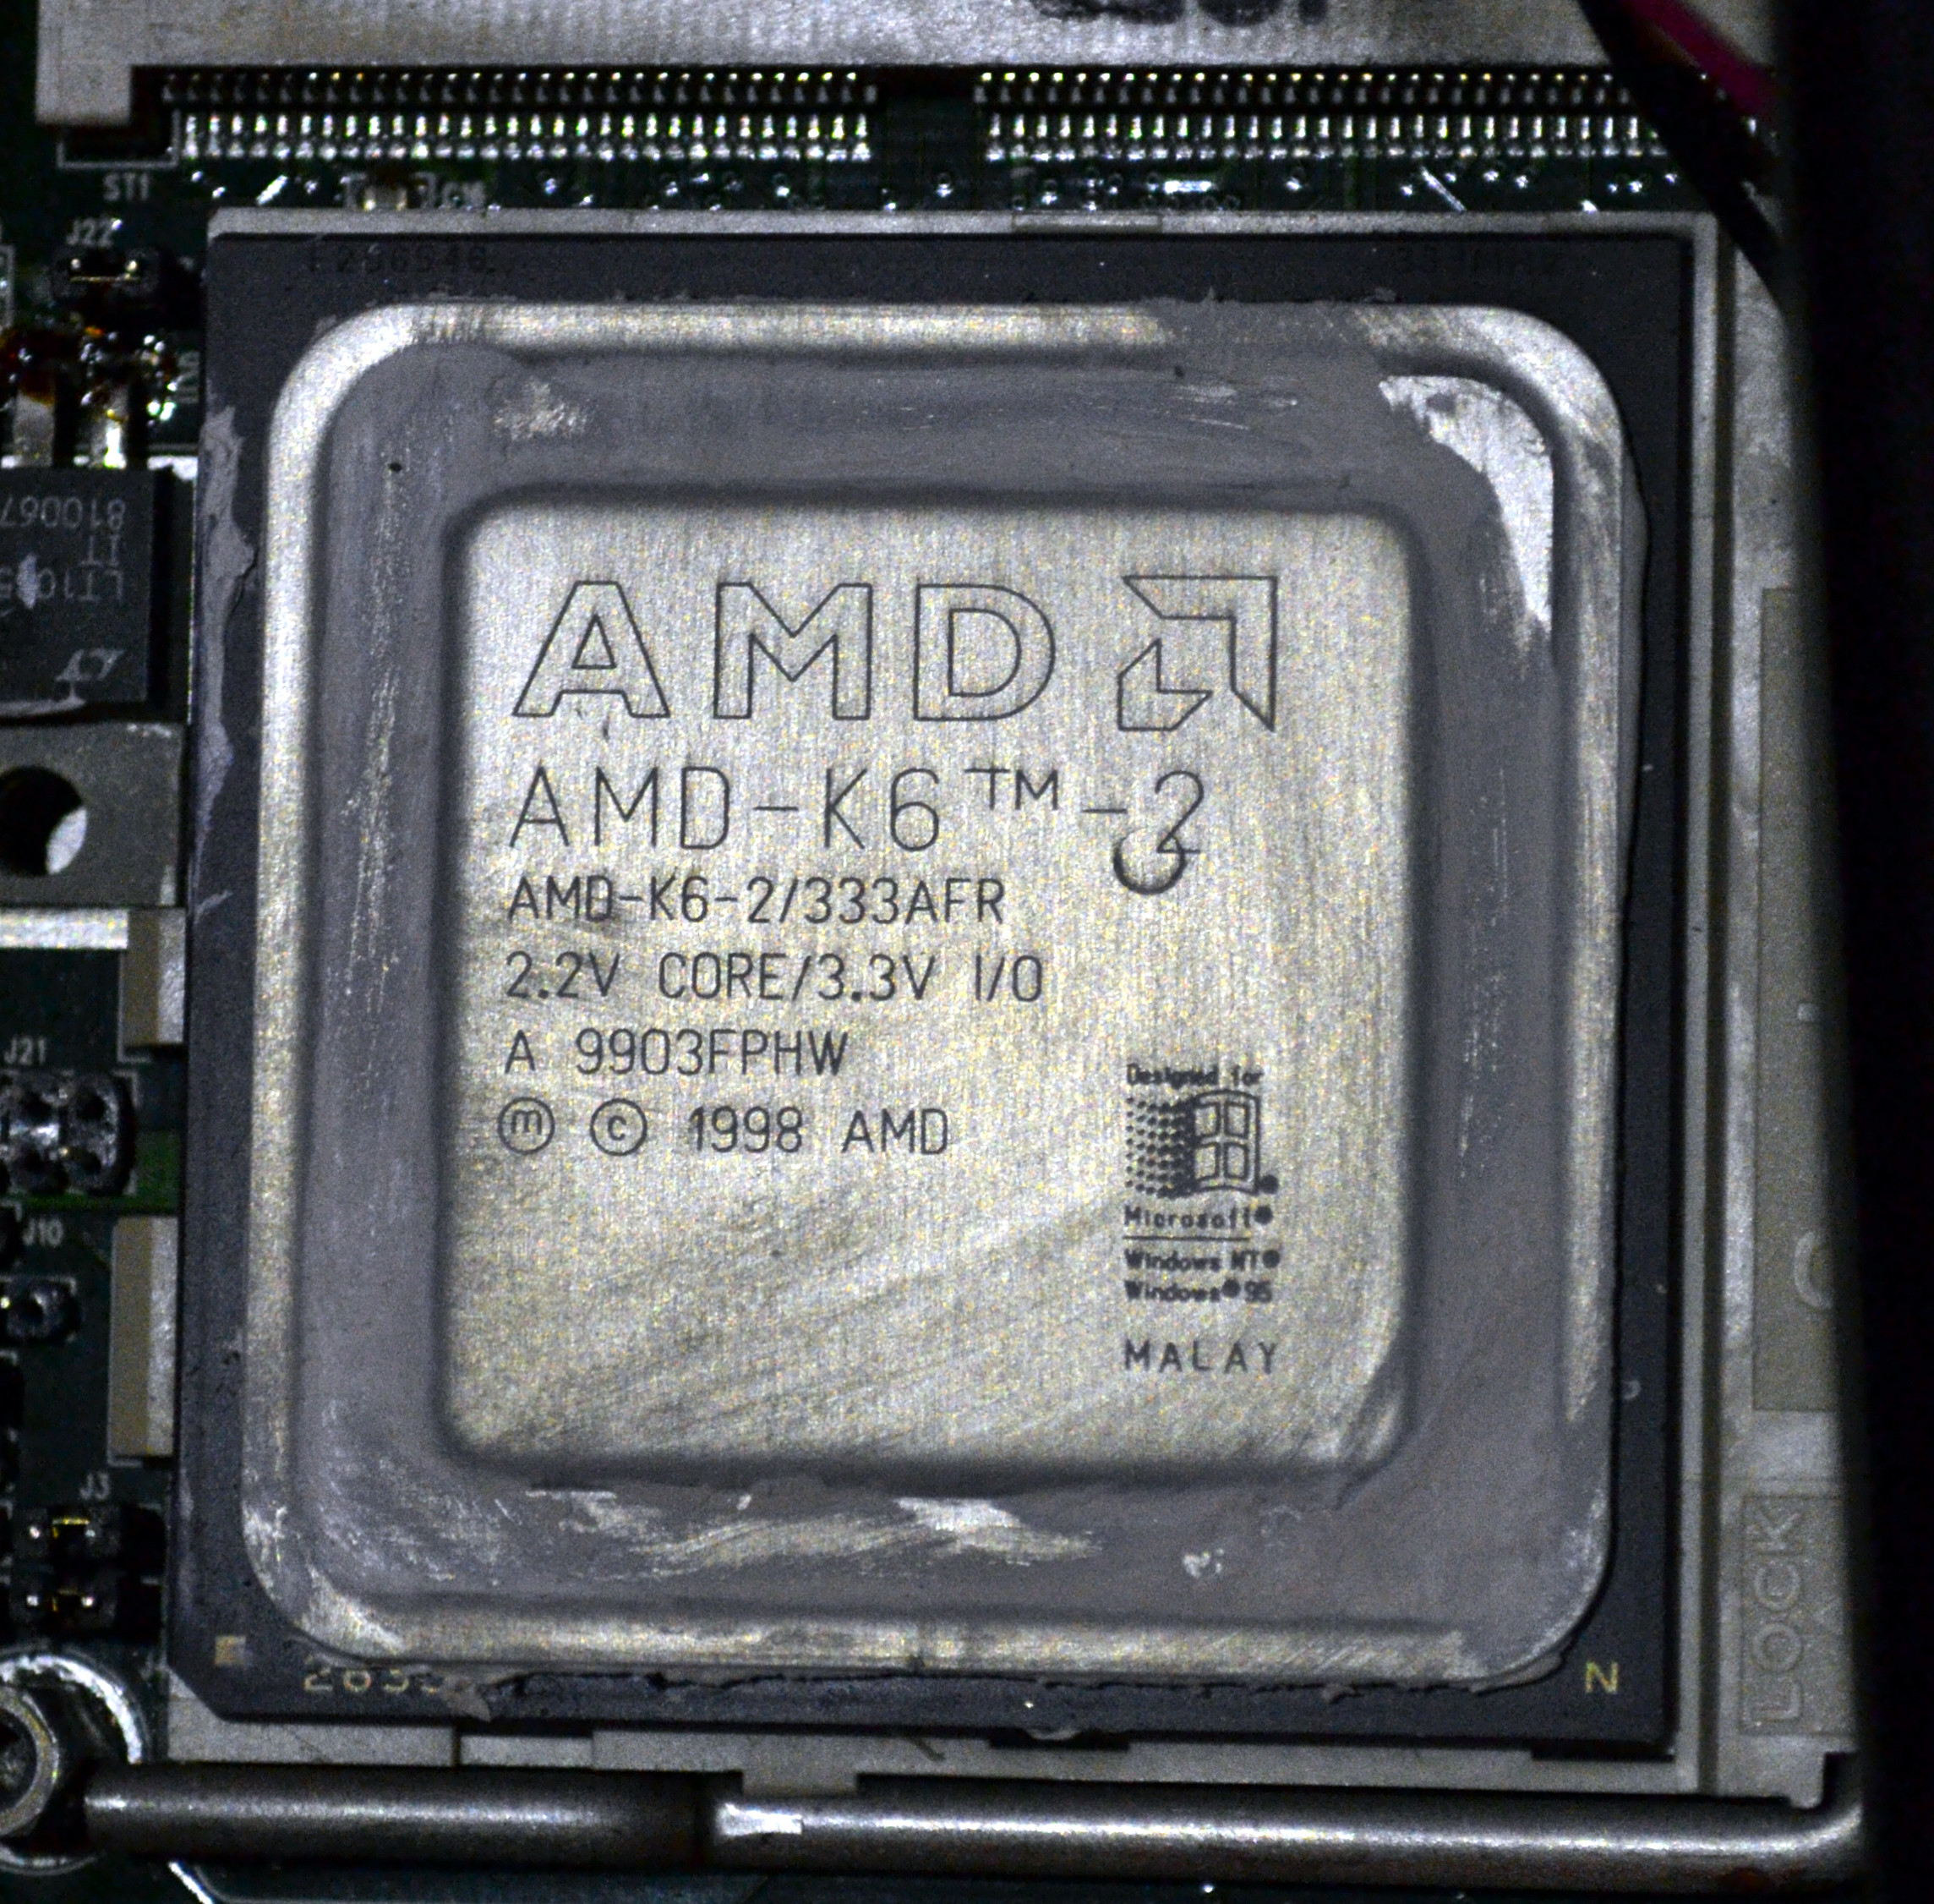
\includegraphics[width=1.000\hsize]{processor.jpg}
\caption{AMD K6 66 MHz}
\end{figure}

Sunitin huolto on ilmoittanut, etteivät he suostu/pysty enää huoltamaan näin vanhaa tietokonetta, mikä on myös osasyynä korvaavien vaihtoehtojen kartoittamiseen.

Sunit Nerosta löytyy 3+1 sarjaporttiliitäntää (3x 9pin standardi RS-232, sekä yksi yhdistetty liitin), rinnakkaisporttiliitin (25pin Centronics), Sunitin oma BUS-liitin PS/2 hiirelle ja näppäimistölle, yhdistetty virta/GPRS/GPS -liitin sekä Data I/O-liitin, joka on tarkoitettu optiona oleville CAN- ja SCSI-väylälle, mutta nämä eivät ole kyseisessä yksilössä käytössä.  Käytössä on kolme sarjaporttia ja virtaliitin. Sarjaporteista yksi on alkuperäiselle Terman-ohjaukselle, yksi Motomit IT:lle ja kolmas on käytöstä poistetulle GSM-moduulille.

Sunit Neroon on ollut lisäoptiona myös GPS ja DGPS-moduulit, jotka olisivat mahdollistaneet kartat paikannuksella. Työn kohteena olevassa yksilössä on GPS-moduuli. Neroon on ollut liitettynä myös ulkoinen GSM-moduuli \cite{nero:manual}. GPS- ja GSM-moduulit eivät ole nykyisessä järjestelmässä käytössä eikä niitä tarvitse ottaa huomioon korvaavassa tietokoneessa.\newline\newline

\begin{figure}[H]
\centering
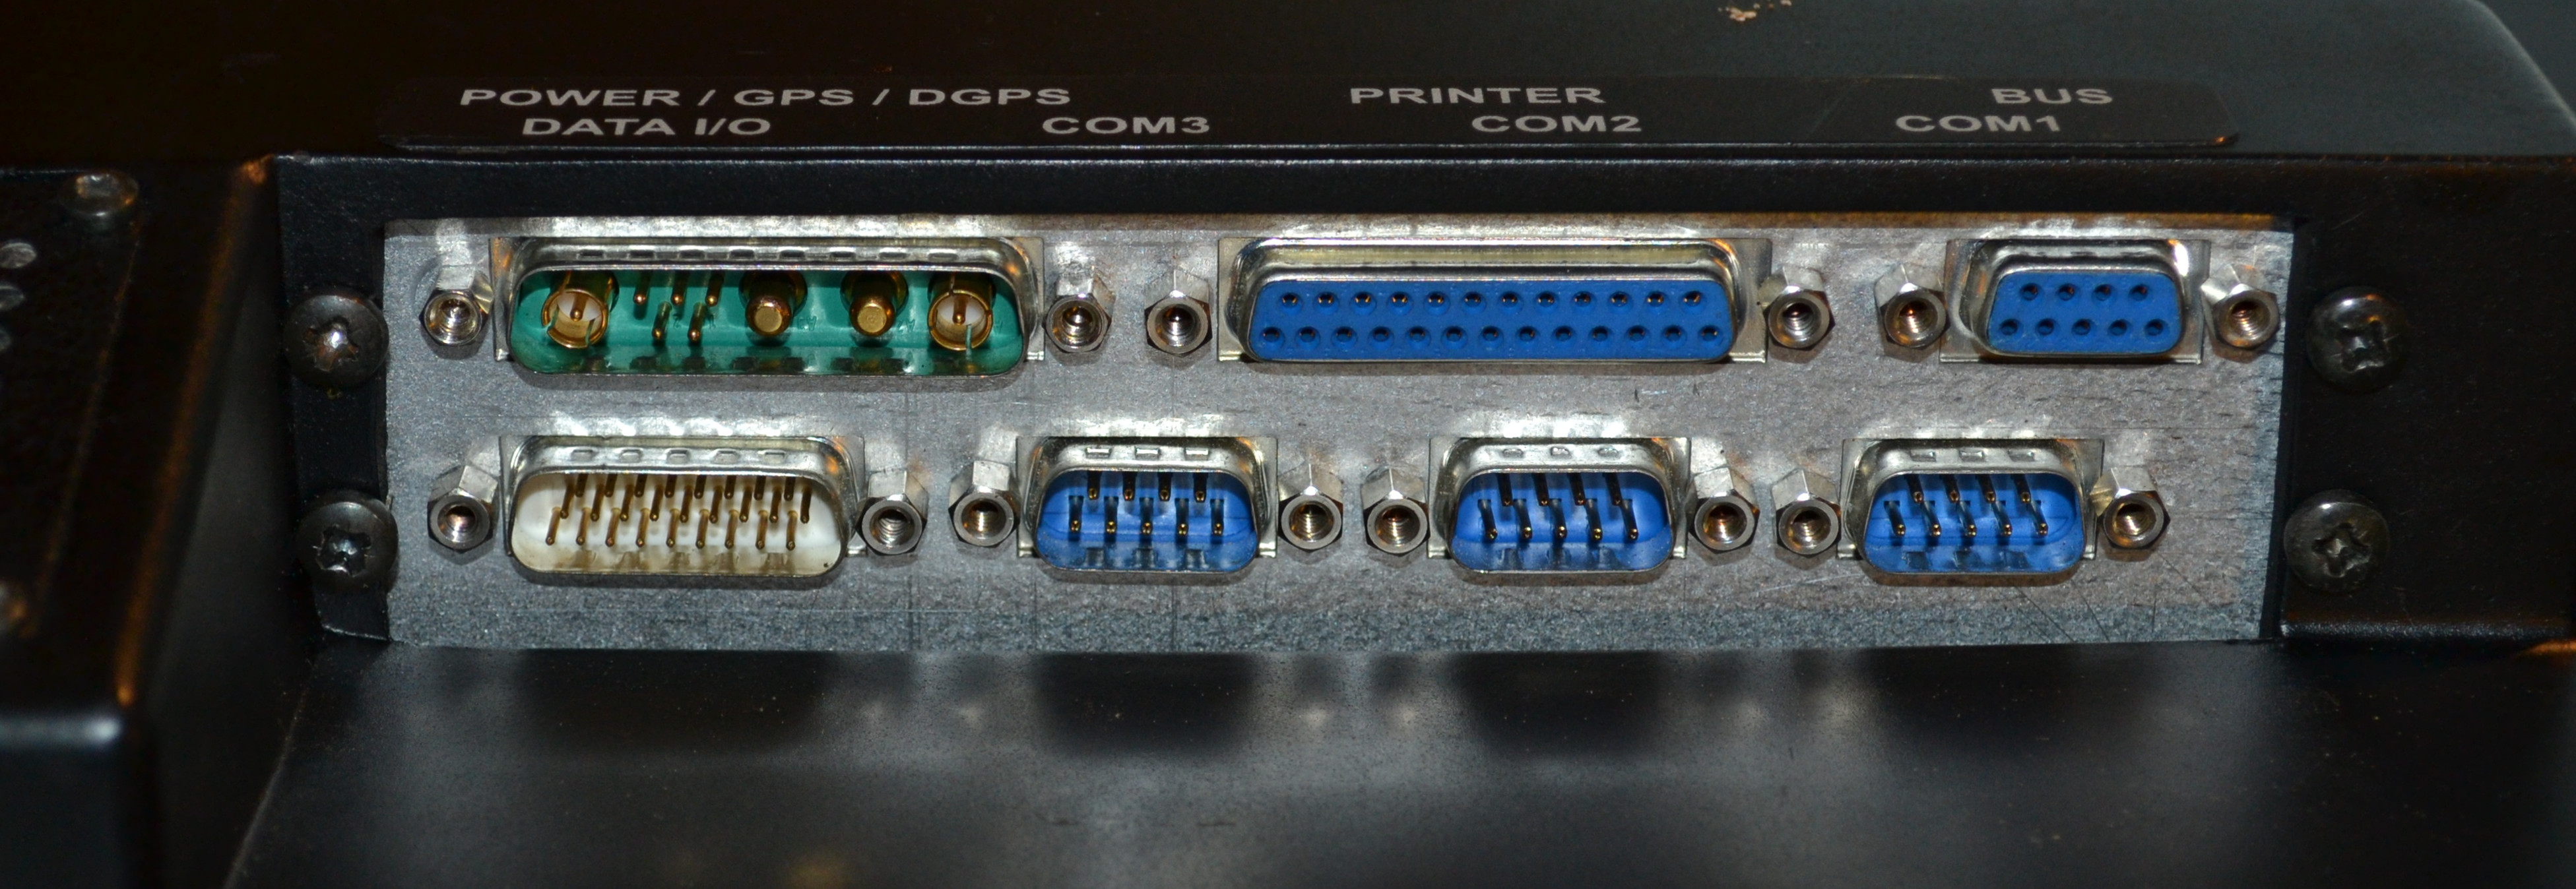
\includegraphics[width=1.00\hsize]{sunit_nero_liitannat.jpg}
\caption{Sunit Neron liitännät}
\end{figure}

Sunit Nero on rakennettu kolmeen kerrokseen kahden 31 cm x 23 cm -kokoisen metallilevyn väliin, joka on ankkuroitu koteloon kiinni neljällä  läpivientiruuvilla. Ensimmäisessä kerroksessa on Neron käyttämä emolevy, keskellä kiintolevy, levykeasema, cd-asema sekä vara-akku. Viimeisessä kerroksessa on 12" LCD -näyttöpaneeli.

\section{Valmet Terman}
Terman on Valmetin alkuperäinen DOS-pohjainen hallinta- ja apteerausohjelmisto käytettävälle hakkuukoneelle. Ohjelmiston versio on riippuvainen käytettävästä hakkuukoneesta. Kommunikointi hakkukoneen kanssa tapahtuu 9600 bitin nopeudella RS-232-sarjaporttia käyttäen. Koska mittauslaite on vaihdettu Motomit IT-järjestelmälle, käytetään Termania lähinnä hakkuukoneen ajo- ja moottoriasetusten hallintaan.
\newline\newline

\begin{figure}[H]
\centering
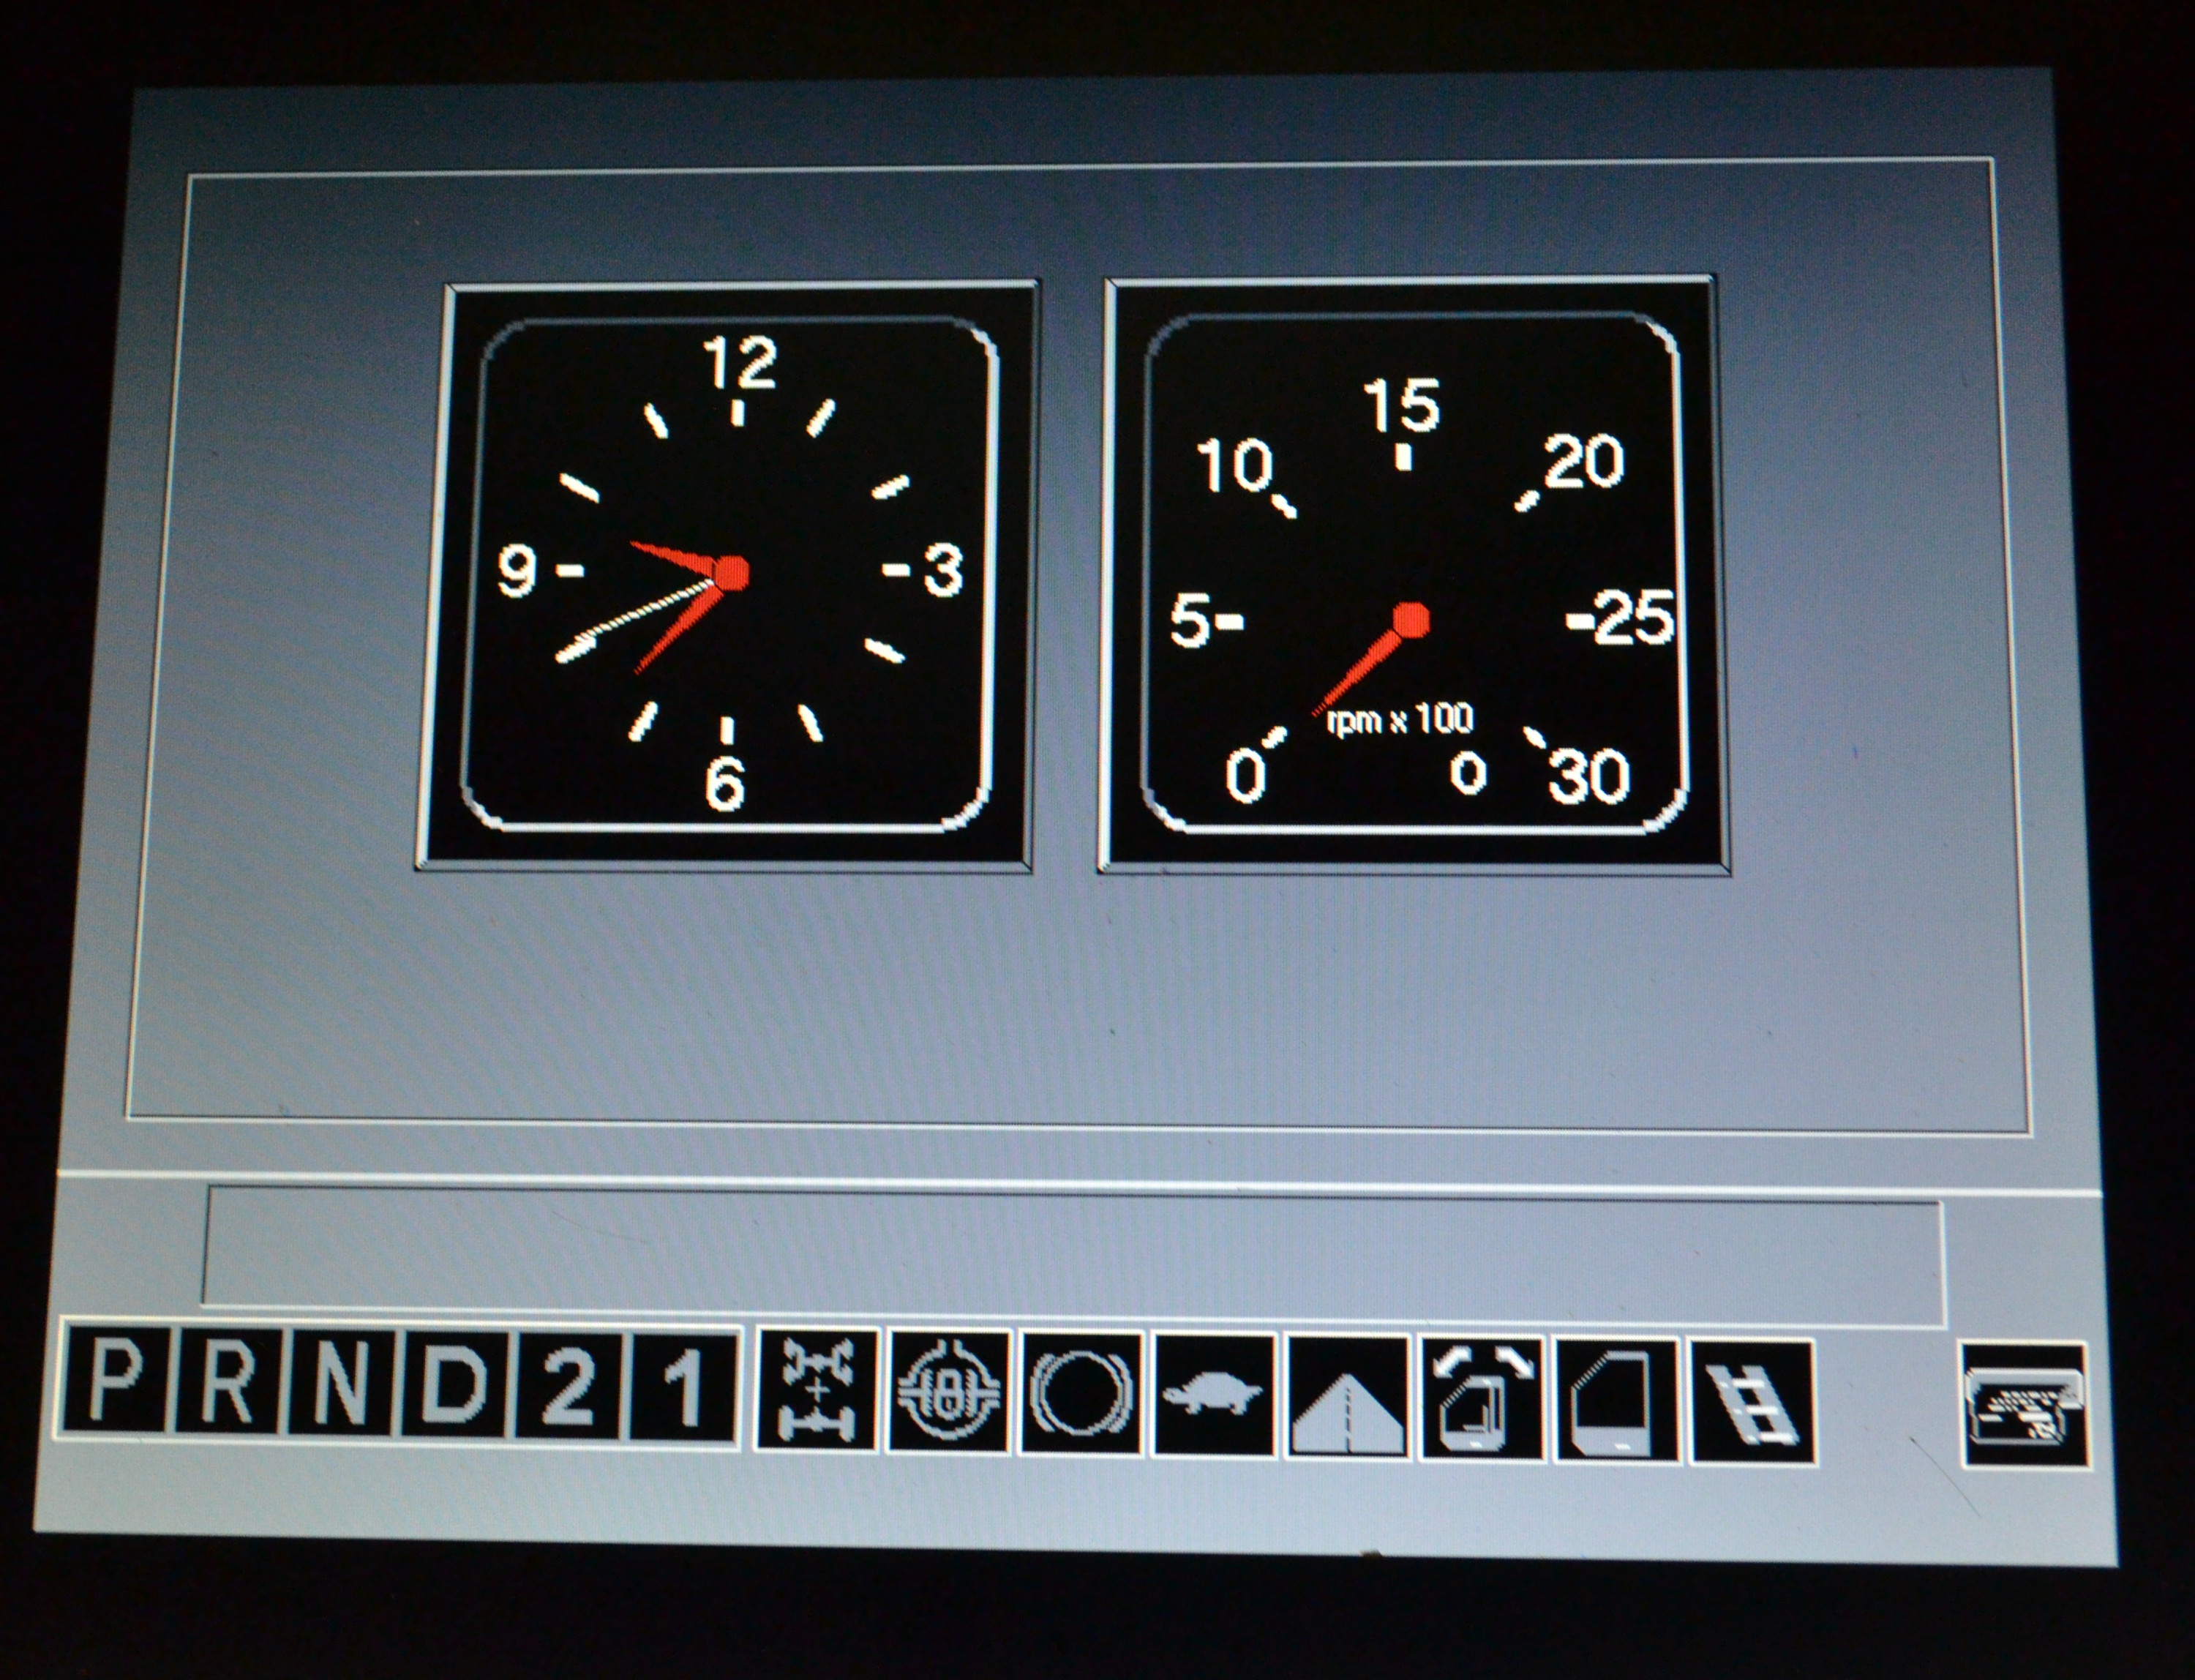
\includegraphics[width=1.00\hsize]{terman_original.jpg}
\caption{Terman Nero-ajoneuvopc:n ruudulla}
\end{figure}

\newpage
\section{Päälohkokaavio}

\begin{figure}[H]
\centering
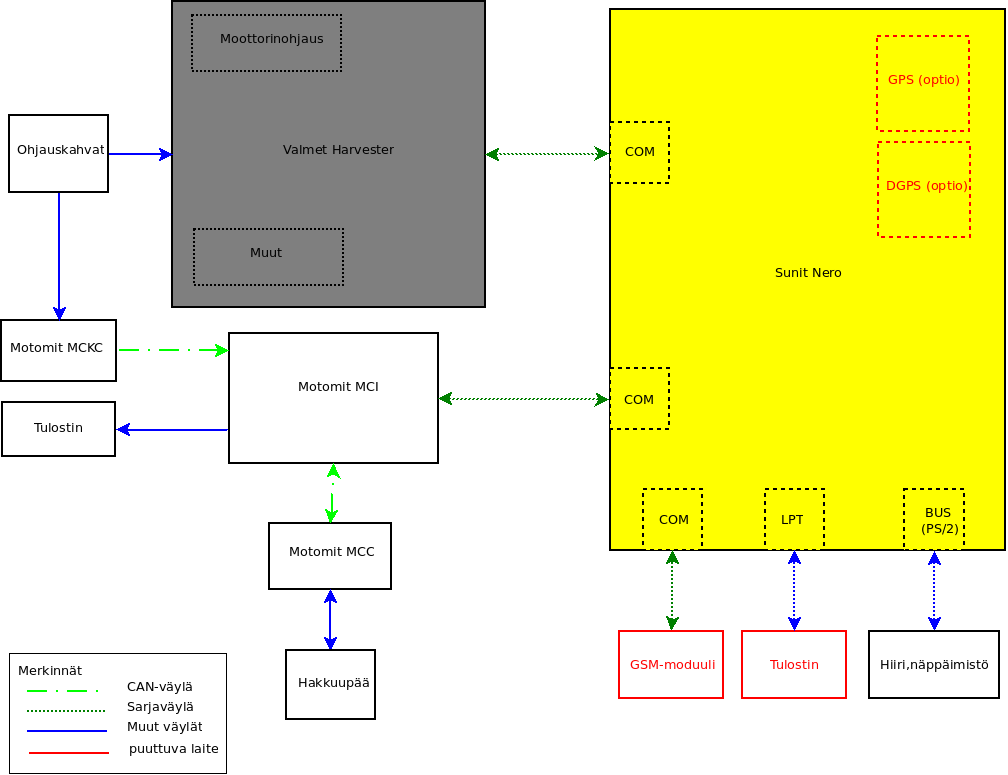
\includegraphics[width=1.00\hsize]{saatanan_kaavio.png}
\caption{Hakkuukoneen järjestelmien lohkokaavio}
\end{figure}

Lohkokaavioon on kuvattu Valmet 901 -hakkuukoneen tärkeimmät osat, niiden käyttämät väylät sekä alkuperäisessä järjestelmässä olleet laitteet. Hakkuukoneessa ei ole itsessään käytössä vielä CAN-väylää, mutta jälkikäteen asennettu hakkuupää, sekä Motomitin mittalaitejärjestelmä käyttää CAN-väylää sisäisesti sekä hakkuupään ohjaukseen. Hakkuukoneen alkuperäiset järjestelmät on ohjattu jokainen laite omalla ohjausjohtimellaan.

% KORJAUSKOMMENTTI
% Onko siis puomin ohjauksessa CAN vai pelkästään hakkuupäässä? Mikä väylä/ohjaustapa niissä osissa on, jotka eivät käytä CAN-väylää?
% -> lisätty

Kaaviosta näkyvistä järjestelmistä ollaan korvaamassa keltaisella näkyvä Nero-ajoneuvotietokone sekä siihen liitetyt hiiri ja näppäimistö.

\newpage
\chapter{Mahdolliset toteuttamisvaihtoehdot ohjelmistojen siirrolle}

Loppukäyttäjän (hakkuukoneen kuljettajan) toiveena on, että tietokoneen vaihtuessa käytössä olevat Terman- ja Motomit PC-ohjelmistot toimivat uudessa koneessa samaan tapaan kuin vanhassa ja näkyvät samalla tavalla kuin ohjelmistot aiemminkin ovat näkyneet. Loppukäyttäjän toiveiden lisäksi on huomioitava tietokoneen käyttöolosuhteiden asettamat vaatimukset sekä aiheeseen liittyvä lainsäädäntö ja standardit.

\section{Natiivi ympäristö}

Natiivilla ympäristöllä tarkoitetaan, että laitteiston ja käyttöjärjestelmän välissä ei ole virtualistointi- tai yhteensopivuusrajapintaa, vaan käyttöjärjestelmällä on suora pääsy fyysisen laitteiston rajapintoihin.

% Natiivin ympäristön hyviä puolia:
% * Suoritusnopeus
% * Ohjelman ja laitteiston välisen kommunikoinnin kutsupolku? lyhyempi
% * toimiessaan yksinkertaisin

% Natiivin ympäristön Haittapuolia ja rajoituksia:
% * Vanhat käyttöjärjestelmät eivät toimi uusien laitteiden kanssa
% ** koska ei löydy laiteajureita
% ** koska uudet laitteet ovat liian nopeita tai liian isolla kapasiteetilla varustettuja suhteessa vanhojen käyttöjärjestelmien toteutuksiin
% * Uudet käyttöjärjestelmät eivät ole välttämättä yhteensopivia vanhojen ohjelmien kanssa
% * (ei liity työhön)
% ** Hyötysuhde huono
% ** Kaikilla ohjelmilla (käyttöjärjestelmästä riippuen) pääsy toisensa tiedostoihin


Natiivin ympäristön vaihtoehdossa ohjelmistoja käytetään ympäristössä, johon ne on aikoinaan suunniteltu toimivaksi. Hyvänä puolena tässä vaihtoehdossa on se, että ohjelmat toimivat varmasti siten kuin ne on suunniteltu. Koska käytettävät ohjelmistot ovat vanhoja, DOS- ja Windows 98- aikaisia, vaatisi natiivin ympäristön käyttäminen kuitenkin suunnilleen samaa alkuperäisen tietokoneen kanssa samaa ikäluokkaa olevan laitteiston käyttämisen. Uudemmat laitteistot eivät ole enää yhteensopivia Windows 98SE / ME:n kanssa ja lisäksi Windows 98:lla on maksimirajoituksia käytettävälle laitteistolle kuten maksimi luotettavasti käytettävä määrä keskusmuistia 1024 Mb ja kiintolevyosiolle rajattu maksimikoko 127,5 Gb \cite{win98:maxspecs}. Uudemmille laitteille ei myöskään löydy välttämättä toimivia ajureita, mikä rajoittaa entisestään mahdollisia laitteistovaihtoehtoja. Koska ajoneuvotietokone ei ole yhdistettynä Internetiin ja koneelle on rajattu pääsy, ei tässä käyttöympäristössä Windows 98:n paikkaamattomilla haavoittuvuuksilla (Windows 98: 84 kpl, Windows 98SE 61 kpl \cite{win98:vulns}) ole erityistä merkitystä käytettävyyteen.

\section{Ohjelmistojen rajapintojen yhteensopivuuskerros}

% Pääpiirteittäin tulkkaa, mutta saattaa virtualisoida joitain laitteistorajapintoja tarvittaessa (näyttö, äänet, HID).
% KORJAUSKOMMENTTI: Yhdistä edelliseen tai jälkimmäiseen kappaleeseen. Yhden lauseen kappaleita ei pidä käyttää.


% Toteutuksia:
% Windows NTVDM DOS ja Windows 3.x -ohjelmia varten
% WOW: a compatibility layer of 32-bit versions of the Microsoft Windows NT family of operating systems that extends the NTVDM to provide limited support for running legacy Win16 applications
%  WoW64 : subsystem of the Windows operating system capable of running 32-bit applications and is included on all 64-bit versions of Windows
%
% Wine (program loader and the Windows API implemented in DLLs)
% Dosemu

% (työhön liittymättömiä)
% Lina -> Linux on MacOSX
% Darling -> OSX on Linux

% vanhoja
% http://en.wikipedia.org/wiki/Wabi_(software)
% https://www.freshports.org/emulators/twin/ , http://gnu.gds.tuwien.ac.at/directory/libs/willowstwin.html


Käyttöjärjestelmän ja ohjelmiston välissä voidaan ajaa erillistä rajapintasovellusta, joka toteuttaa toisen käyttöjärjestelmän järjestelmäkirjastot ja järjestelmäkutsut ja mahdollistaa näin muuten yhteensopimattomien, mutta samaa prosessoriarkkitehtuuria käyttävien ohjelmistojen suorituksen \cite{ntvdm_kb}. Ohjelmistojen rajapintojen yhteensopivuuskerros-vaihtoehdossa  käytetään käyttöjärjestelmän ja ohjelman välissä sopivia rajapintakerroksia, jolloin saadaan käyttöjärjestelmän kanssa yhteensopimattomat ohjelmat toimimaan keskenään. Vaihtoehto vaatii yhteensopivan laitteistoarkkitehtuurin alkuperäisen järjestelmän kanssa (x86). Nykyiset Windows-versiot (Windows XP+) sisältävät jo valmiiksi yhteensopivuustilan, joka mahdollistaa vanhempien ohjelmien käyttämisen uudemmissa käyttöjärjestelmissä. Linuxissa Wine-rajapinta mahdollistaa kaikenikäisten Windows-sovellusten ajamisen Linuxissa. Myös DOS:lle löytyy rajapintakerrostoteutus Linuxiin.

\subsection{NTVDM ja WOW}
%https://kb.iu.edu/d/acxn
%https://technet.microsoft.com/library/cc767884.aspx

Virtual Dos Machine on teknologia, mikä mahdollistaa DOS-ohjelmien suorituksen muissa käyttöjärjestelmissä. VDM -toteutuksia löytyy niin Windowseista 3.x -käyttöjärjestelmästä lähtien, OS/2 sisälsi hyvän DOS-tuen oman MVDM -toteutuksensa takia. VDM on toteutettu myös Wineen lähinnä 16 -bittisten Windows 3.x -ohjelmien tuen takia. 16-bittisten ohjelmien tukea tarvitaan työssä TERMAN-ohjelmistolle.

NTVDM NT Virtual DOS Machine ja WOW Windows On Windows ovat Windows -käyttöjärjestelmän alijärjestelmiä, jotka DOS- ja 16 -bittisten Windows 3.x -ohjelmien suorittamisen uudemmissa NT -kerneliin pohjautuvissa Windows -versioissa. NTVDM oli toteutettu emulaattorina myös Windows NT:n MIPS- ja Alpha-versiolle . NTVDM ja WOW on poistettu 64 -bittisisistä Windows -versioista. \cite{ntvdm_2}

NTVDM emuloi x86-prosessorin suorittamassa MS-DOS -käyttöjärjestelmää. Se tulkkaa DOS-ohjelmien tekemät suorat laitteiston manipulointipyynnöt Windowsin API-pyynnöiksi. Emuloitujen laitteistojen tuki on kuitenkin NTVDM:ssä yksinkertainen ja rajoittunut. Se ei rajaa ohjelmien suoritusnopeutta, jolloin moni DOS-ohjelma pyörii nykylaitteistolla liian lujaa eikä kommunikointi laitteiston kanssa välttämättä onnistu koska ohjelmat eivät odota vastausta tarpeeksi pitkään.

NTVDM:n ratkaisu DOS:n tietoturvaongelmiin on ajaa jokaista DOS-ohjelmaa omassa VDM-prosessissa, jolloin ohjelmat ovat suojattuja toisiltaan. DOS-ohjelmien kaatuminen ei vaikuta muihin ohjelmiin / suoritettaviin prosesseihin, koska jokainen suoritettava DOS-ohjelma on oma VDM-prosessinsa. Uudemmissa käyttöjärjestelmissä (Windows 7+) voi määritellä ajetaanko ohjelmat omina prosesseinaan vai yhden VDM-prosessin alla.

WOW, Win16 on Win32, on Windowsin alijärjestelmä joka täydentää NTVDM:ään tuen 16 -bittisille Windows -ohjelmille. Win16 -ohjelmat ajetaan yhdessä VDM -prosessissa omina säikeinään. Tällä tavoin on saatu aikaan paras yhteensopivuus Windows 3.x:n kanssa. Haittapuolena tulee jaettu muistiavaruus kaikkien 16 -bittisten ohjelmien kanssa joka voi aiheuttaa epävakautta alijärjestelmän sisällä. Alijärjestelmän kaatuminen sulkee kaikki 16 -bittiset ohjelmat, muttei vaikuta käyttöjärjestelmän toimintaan muuten. \cite{ntvdm_kb}


\subsection{Wine}
%https://www.winehq.org/docs/winedev-guide/x2884
Wine on POSIX-yhteensopiville käyttöjärjestelmille kehitetty yhteensopivuuskerros, jolla 32- ja 64-bittiset Windows-ohjelmat saadaan toimimaan muissa käyttöjärjestelmissä. Wineen on toteutettu Windowsin kernelin järjestelmäkutsut, sekä useita tarvittavia DLL-kirjastoja. Työssä tarvitaan 32-bittistä Windows-tukea Motomitin hallintaohjelmistolle.

Wineen pystyy asettamaan käyttöön tarvittaessa alkuperäisen järjestelmän jaettuja DLL-kirjastoja. Alkuperäinen DLL tarjoaa täyden yhteensopivuuden kirjaston toteuttamille rutiineille. Näiden käytön vaarana on, että ne voivat yrittää käyttää Windowsin järjestelmäkomponentteja joita Wineen ei ole toteutettu, jolloin toiminnallisuus kärsii. Winen sisäänrakennetut DLL:t sisältävät tarvittavilta osin lisäyksiä ja välityskoodia / käärekoodia joilla kirjastot saadaan toimimaan Unixissa käytetyjen ratkaisuiden kanssa yhteen.

Wine ei tue Windowsin ajurien käyttöä, koska Winen kernel-ratkaisut eivät sisällä tähän mahdollisuutta. Wine tukee joitain laitteita, jos ja vain jos niille löytyy käytettävästä käyttöjärjestelmästä ajurituki, sekä itse Wineen on toteutettu tarvittavat rajapintamuunnokset kyseiselle laitteelle. Winessä on kuitenkin ohitettu ajurien tarve toteuttamalla monet DLL-kirjastot siten, että ne käyttävät Unixin rajapintoja (tulostus, äänet, näyttö). Jokainen Wine-prosessi (==suoritettava exe) ajetaan omana prosessina, jolloin niillä on omat osoiteavaruudet (eivätkä ne voi sörkkiä toisetensa muistia).

Winen kehitys alkoi jo vuonna 1993, kun Bob Amstadt halusi suorittaa sen aikaisia Windows 3.1 -ohjelmia Windowsin puolella. Kehitysvastuu v. 1994 Alexandre Julliard:lle, joka on toiminut Wine Projectin johtohahmona ja projektin vetäjänä siitä lähtien. Winen koodista n. puolet on kirjoitettu vapaaehtoisten toimesta. Yrityspuolelta projektin pääasiallinen sponsori on CodeWeavers, jonka työntekijöitä myös moni Wine-kehittäjä on. CodeWeavers on kehittänyt CrossOver linux-tuotteensa joka on kaupallistettu, käyttäjäystävällisempi versio Winestä. CodeWeavers tarjoaa myös ohjelmistojen porttaus- ja tukipalveluita Winelle.

Winen 1.0 -versio julkaistiin vuonna 2008. Winestä julkaistaan uusi vakaa (stabiili, virallinen, tuettu, jotain) versio kahden vuoden välein. Viimeisin vakaa versio on 1.6. Wine käyttää versionumeroinnissaan sekventiaalista Major.Minor.Build -tyyliä, jossa parilliset Minor-versiot ovat vakaita julkaisuita ja parittomat kehitysversioita.


\begin{figure}[H]
\centering
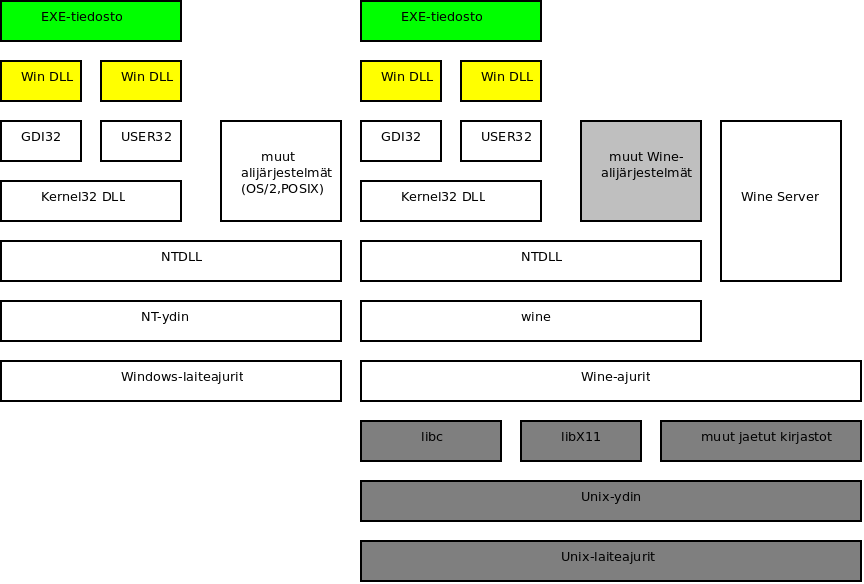
\includegraphics[width=1.00\hsize]{kaaviot/wine_pino.png}
\caption{Vasemmalla Windows NT:n käyttämä arkkitehtuuri, oikealla Wineen toteutettu arkkitehtuuri}
\end{figure}

Wine serverin avulla on totetutettu IPC:n (prosessien välinen kommmunikointi), synkronointi, ja prosessien/säikeiden hallinta. Windows-alijärjestelmistä on toteutettuna vain Win32-alijärjestelmä (Kernel32). Winen toteuttamien DLL-tiedostojen nimeämiskäytäntö on pyritty pitämään mahdollisimman lähellä Windowsin nimeämiskäytäntöä, jos vain se on ollut mahdollista. \cite{wine:architecture}

\subsection{Dosemu}
% Mikä doesmu
%mitä tulkitaan
% mitä emuloidaan

Dosemu on Linuxille kehitetty yhteensopivuuskerros, jolla saa ajettua 16-bittisiä DOS-ohjelmia x86/x64-arkkitehtuuria käyttävässä Linux-käyttöjärjestelmässä. Dosemu on käyttäjätason ohjelma (ei vaadi pääkäyttäjän/root-oikeuksia), joka hyödyntää 80386:n ja Linux -kernelin erityisominaisuuksia ajaakseen DOS-ohjelmia eriytettynä prosesseina. Dosemu virtualisoi kaiken i/o-liikenteen, simuloi laitteistoa johon DOS-ohjelmilla on suora pääsy, sekä tarjoaa virtuaalisen kiintolevyn joka oikeasti on tiedostopolku Linuxissa. Dosemu on yhtenä mahdollisuutena TERMAN-ohjelmiston suorittamiseen kohdejärjestelmässä.

Tekstipohjaiset DOS-ohjelmat saa suoritettua DOSEMU:n avulla suoraan konsolissa, mutta siitä löytyy myös CGA/EGA/VGA-emulaation DOS:n graafista moodia käyttäville ohjelmille(Mode 13h 320x200 256 väriä). Dosemu sisältää myös tuen sarja- ja rinnakkaisporteille.

% http://www.dosemu.org/docs/HOWTO/x596.html#AEN598
Dosemun kehitys alkoi v. 1992 Matthias Lautnerin toimesta. Projekti vastuuhenkilö vaihtunut vuosien varrella ja vuodesta 2004 lähtien vastuussa on ollut Bart Oldeman.

%Tähän vitun hieno kaavio? DOS on kyllä niin aneeminen että en tiedä löytyykö



\section{Virtualisointi}

Tässä vaihtoehdossa alkuperäisiä ohjelmistoja+käyttöjärjestelmää ajetaan virtuaalikoneessa toisen käyttöjärjestelmän päällä. Näin saavutetaan varmin yhteensopivuus ohjelmistotasolla. Oheislaitteiden siirtämisessä virtualisoidun koneen käyttöön on rajoituksia, jotka pitää huomioida virtualisointiohjelmistoja valittaessa. Vaihtoehto kuluttaa muistia enemmän ja on hieman hitaampi kuin natiivi toteutus, hyötysuhteen ollessa \textasciitilde{}90\%  natiivista \cite{virtnat_anadtech}.

%KORJAUSKOMMENTTI: Viittaa lähteeseen!
% KKOMMENTTI: Lähdeviittaukset olemassa, ei docx:ssä

Virtualisoinnin ollessa varsin yleistä, niin virtualisointiratkaisuita tarjoavia yrityksiä ja ohjelmistoja on paljon. Työpöytävirtualisointiin riittävillä ominaisuuksilla (mm. sarjaporttien välitys virtuaalikoneille) sopii esimerkiksi avoimen lähdekoodin QEMU-hypervisori tai Oraclen Virtualbox -hypervisori. Myös Microsoft tarjoaa Windows-ympäristöön VirtualPC-hypervistoria. Kaupallisista tarjoajista VMWarella on olemassa VMWare Workstation ja VMWare Player -hypervisori. Virtualisoinnin avulla pyritään ajamaan alkuperäisen ajoneuvotietokoneen Windows 98 -käyttöjärjestelmää, sekä ohjelmia, ilman erillisiä rajapintakerroksia.

Hypervisorit on jaettu kahteen tyyppiin, 1 -tyypin natiiveihin hypervisoreihin joita ajetaan laitteiston ja käyttöjärjestelmän välissä, sekä 2-tyypin \"hosted\" -hypervisoreihin jotka suoritetaan tavallisina ohjelmina käyttöjärjestelmästä. Tämä jako ei kuitenkaan ole kaikkien hypervisoreiden kohdalla näin selvä (wink wink KVM)


\subsection{Virtuaalikoneet}
\subsubsection{Xen}
%http://wiki.xenproject.org/wiki/Xen_Overview
%QEMU is involved only in the emulation of hardware; the execution of the guest is done within Xen and is totally hidden from QEMU.
Xen on Cambridgen yliopistossa kehitetty 1-tyypin hypervisor/virtuaalikone. % http://www.xenproject.org/about/history.html
Xenin kehitystyö aloitettiin 1990-luvun loppupuolella Xenoserver -projektin yhteydessä ja ensimmäinen julkinen avoin versio julkaistiin lokakuussa 2003, jonka jälkeen uusia versioita on julkaistu säännöllisesti, uusimman ollessa v. 4.5. \cite{xen_history} Xen suoritetaan käynnistyslataimesta (bootloaderista), jolloin se asettautuu laitteiston ja virtuaalikoneiden väliin. Xen vaatiikiin aina suoritettavaksi yhden virtuaalikoneen eli ns. isäntäkoneen eli Dom0:n. Dom0 hoitaa interaktion laitteiston sekä muiden virtuaalikoneiden kanssa. Lisäksi ainoastaan Dom0:lla on pääsy Xenin rajapintaa jota kautta hallitaan järjestelmää.

Xen vaatii erillisen tuen kohdekäyttöjärjestelmiltä jotta niitä voidaan käyttää Xenin avulla paravirtualisoituina (pl. rautatason virtualisointi jolloin kohde ei tarvitse muutoksia). Tuki Xenin paravirtualisoinnille löytyy kuitenkin useimmista Linux- ja BSD-jakeluista. Windowsissa ei ole tukea Xenin paravirtualisoinnille, mutta sitä voidaan ajaa laitteistoavusteisen virtualisoinnin avulla Xenin päällä. Xen on tarkoitettu palvelinten virtualisointiin ja siten sen ratkaisut ja toteutus tekevät siitä epäkäytännöllisen tätä projektia ajatellen. \cite{xen_overview}

%The Control Domain (or Domain 0) is a specialized Virtual Machine that has special privileges like the capability to access the hardware directly, handles all access to the system’s I/O functions and interacts with the other Virtual Machines. It also exposes a control interface to the outside world, through which the system is controlled. The Xen Project hypervisor is not usable without Domain 0, which is the first VM started by the system.

\begin{figure}[H]
\centering
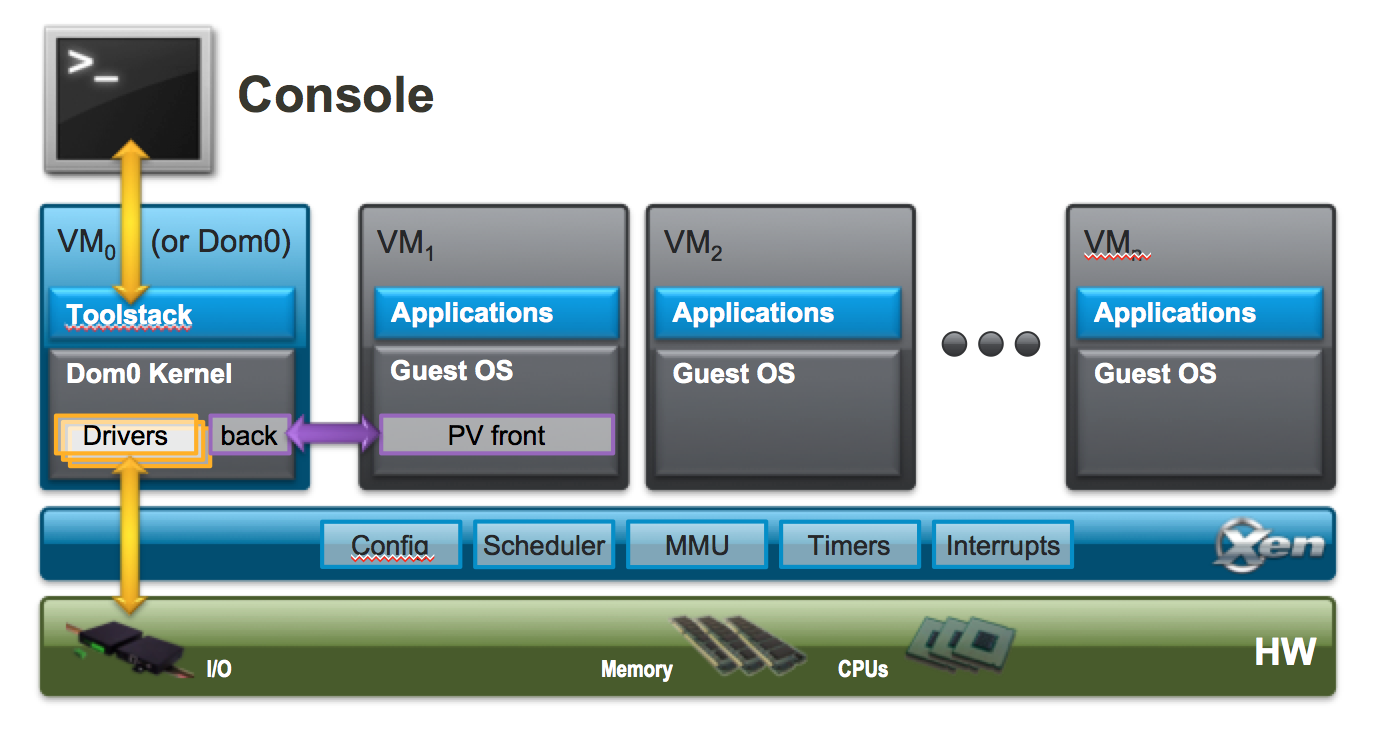
\includegraphics[width=0.60\hsize]{Xen_Arch_Diagram.png}
\caption{Xenin arkkitehtuurikaavio.}
\end{figure}

\subsubsection{KVM}
%http://www.linuxthoughts.com/?p=110
%https://www.youtube.com/watch?v=6n-ANRWqll8
KVM (Kernel Mode Virtualization) on Linux-ytimeen rakennettu tuki virtualisoinnille. KVM vaatii prosessorilta virtualisointituen. KVM ei itsessään emuloi mitään, vaan tarjoaa käyttäjätasolle rajapinnan prosessorin virtualisointiominaisuuksiin. KVM on toteutettu siten, että se että oikeastaan muuttaa Linux-kernelin hypervisoriksi/virtuaalikoneeksi hyödyntäen muita Linuxin komponentteja, kuten vuorottelijaa, sekä muistinhallintaa. \cite{kvm1}

% http://www.linux-kvm.org/wiki/images/6/61/KvmForum2007$kf2007-keynote.pdf
KVM:n kehitys alkoi v. 2006 \cite{kvm3}, Ensimmäinen vakaa, Linuxin kernelin mukanaa toimitettava versio julkaistiin syyskuussa 2012. KVM koostuu kernel -moduulista kvm.ko joka toteuttaa virtualisoinnin perusrakenteet, prosessoririppuvaisista kernel-moduuleista (esim kvm-intel.ko ja kvm-amd.ko.) sekä käyttäjätason ohjelmasta (qemu-system-ARCH) joka emuloi laitteiston ja toteuttaa virtuaalikoneiden (guest) hallinnan. Jokaiselle virtuaalikoneelle emuloidaan omat laitteistot. Alussa hallintaan käytettiin muunneltua QEMU:n versiota, mutta QEMU 1.3:sta lähtien tarvittavat muutokset on lisätty QEMU:un. KVM:lle ei toistaiseksi ole toteutettu muita käyttäjätason hallintaohjelmia kuin QEMU. QEMU:n päälle on kuitenkin toteutettu laaja joukko hallintaohjelmia (libvirt). \cite{kvm2}


%https://www.suse.com/documentation/sles-12/book_virt/data/sec_kvm_intro_arch.html
\begin{figure}[H]
\centering
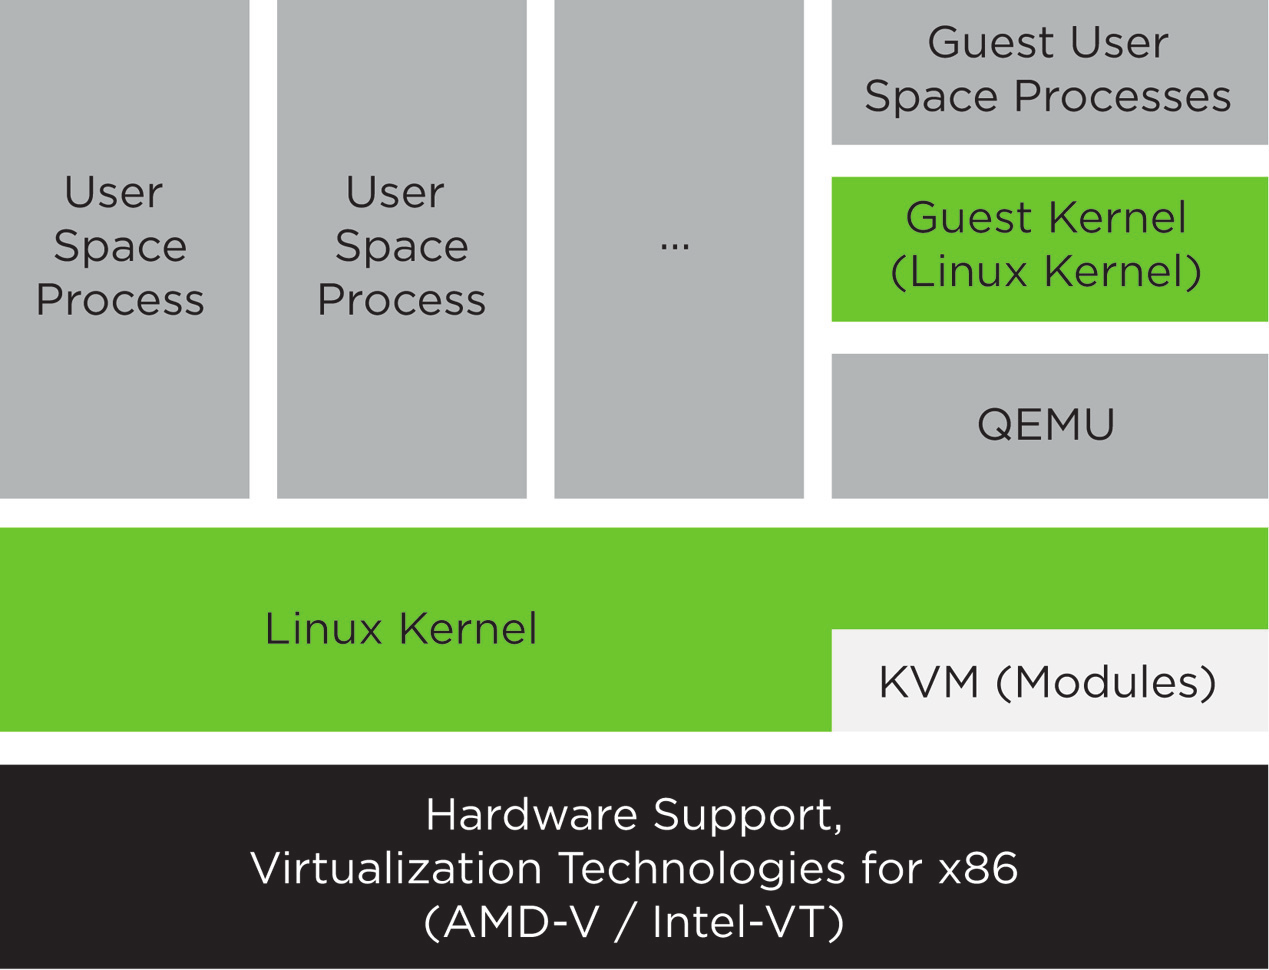
\includegraphics[width=0.60\hsize]{kvm_qemu.png}
\caption{KVM:n arkkitehtuurikaavio.\cite{kvm4}}
\end{figure}

\subsubsection{Oracle Virtualbox}

Oracle Virtualbox on henkilökohtaisessa käytössä ilmainen virtuaalikone Windows-, sekä *NIX-käyttöjärjestelmille. Se toimii 2-tason hypervisorina (käyttöjärjestelmän päällä ajettavana virtuaalikoneena) ja tukee x86- sekä x64 -käyttöjärjestelmien virtualisointia \cite{virtualbox_manual}. Virtualboxin perusohjelmisto on GPLv2-lisensoitua ja siihen tarjotaan  PUEL-lisenssoituja suljetun lähdekoodin lisäpaketteja. Virtualboxin ensimmäinen versio julkaistiin 15.1.2007 yrityksen Innotek GmbH toimesta. Sun Microsystems Inc. osti Innotekin helmikuussa 2008. Oracle Corporation osti Sun Microsystemsin 27.1.2010 ja vastaa Virtualboxin myynnistä ja kehityksestä.


%With version 4 of VirtualBox, released in December 2010, the core package is free software released under GNU General Public License version 2 (GPLv2). This is the fully featured package, excluding some proprietary components not available under GPLv2.
%https://www.virtualbox.org/wiki/VirtualBox_PUEL
%https://www.virtualbox.org/wiki/Licensing_FAQ
%Personal use is when you install the product on one or more PCs yourself and you make use of it (or even your friend, sister and grandmother). It doesn't matter whether you just use it for fun or run your multi-million euro business with it. Also, if you install it on your work PC at some large company, this is still personal use. However, if you are an administrator and want to deploy it to the 500 desktops in your company, this would no longer qualify as personal use. Well, you could ask each of your 500 employees to install VirtualBox but don't you think we deserve some money in this case? We'd even assist you with any issue you might have.

Virtualbox on ilmainen koti- ja arviointikäyttöön. Oracle myy Enterprise-versiota n. 50 USD hintaan.
Virtualboxin PUEL-lisenssin mukaan Virtualboxin ilmaisen version käyttö on sallittua kaupallisestikin jos ohjelmiston asennus ja käyttö on yksittäisen henkilön hallittavissa. Maksullinen Enterprise -versio tarvitaan jos ohjelmistoa toimitetaan esiasennettuna tai sen asennusta ja käyttöä vaaditaan tai hallitaan yritystasolla.\cite{virtualbox_puel}\cite{virtualbox_licensing}

Virtuaalikoneita hallitaan sekä Virtualboxin graafisella käyttöliittymällä, että VBoxManage -komentoriviohjelmistolla joka tarjoaa graafinen käyttöliittymän ominaisuuksien lisäksi pääsyn kaikkiin virtualisointimoottorin ominaisuuksiin\cite{virtualbox_manual}. Virtualboxin ominaisuuksiin kuuluu mm. virtuaalikoineiden moniprosessorituki, USB-laitteiden tuki, sekä snapshotit. Virtualbox tukee 2 sarjaportin välittämistä kohdejärjestelmälle. Lisäksi VirtualBoxista löytyy version Windows-, Linux-, OSX-, (Open)Solaris-, sekä FreeBSD-käyttöjärjestelmille. Virtualboxin puutteita ovat rajoittunut virtuaalikoneiden verkonhallinta useiden virtuaalikoneiden tapauksessa, USB 3.0- tuen puuttuminen sekä sisäkkäisten virtuualikoneiden ajon tuki \cite{vplayervsvbox}.


\subsubsection{VMWare Player}
VMWare Player on VMWare Inc.:n v. 2008 julkaistu kaupallinen virtualisointiohjelmisto. Uusin versio on joulukuussa 2014 julkaistu 7.0. VMWare Player on kotikäyttöön ilmainen, mutta kaupallinen käyttö vaatii lisenssin hankkimisen. VMWare Player käyttää samaa virtualisointiydintä VMWare Workstationin kanssa, josta riisuttu versio Player oikeastaan on. VMware playerin ominaisuuksiin kuuluu 4 sarjaportin välitys kohdejärjestelmälle, xxxxxxxx. Laitteiston välitystuki on suht. hyvä Playerissa . VMware Playerista on versiot Windows- ja Linux -käyttöjärjestelmille. \cite{vmware1}


Playerista puuttuu snapshotit, ja siinä on hyvin rajoittunut komentorivi -käyttöliittymä. Suoritusnopeudessa VMware Player voittaa Virtualboxin pienellä erolla.\cite{vplayervsvbox}


% Blaah. Esittely QEMUsta, Virtualboxista, VirtualPC:stä, VMWaren shaibasta
%http://qemu.weilnetz.de/qemu-tech.html#intro_005ffeatures
\subsection{QEMU}
QEMU (Quick Emulator) on avoimen lähdekoodin emulaattori ja virtuaalikone, joka toimii Linuxin lisäksi myös Windowsissa ,sekä Mac OS X:ssä. QEMU tukee erilaisia toimintamoodeja. QEMU:n rakenne on jaettu backendiin, joka vastaa isäntäkoneen arkkitehtuurituesta, sekä frontendiin, joka vastaa kohdeprosessorin emuloinnin toteuttamisesta. Tällä rakenteella on saatu aikaiseksi järjestelmä, joka on sekä helppo portata sekä johon on helppo toteuttaa uusia prosessoreita eri käskykannoilla. \cite{qemu_doc}

%http://qemu.weilnetz.de/qemu-tech.html#QEMU-compared-to-other-emulators
QEMU käyttää dynaamista käännöstä (dynamic translation) nopeuttakseen emulointinopeutta. Dynaamisessa käännöksessä tulkitaan ja käännetään ajettavaa tiedostoa pieni osa, blokki, kerrallaan. Blokki on haarautumiseen ja hyppykäskyihin asti oleva pätkä käskyjä. Koska yleensä dynaamiset kääntäjät ovat monimutkaisia ja arkkitehtuurisidonnaisia, on QEMU:n kääntäjä TCG (Tiny Code Generator) pidetty yksinkertaisena ja helposti siirrettävänä (portattavana). TCG:n perusidea on jakaa jokainen käsky TCG:n RISC-tyylisiksi käskyiksi, jotka sitten muutetaan kohdejärjestelmän käskyiksi. \cite{qemu_tech}
%Dynaamisessa muutoksessa kakataan koodin päälle ja toivotaan ettei kukaan huomaa.
%http://git.qemu.org/?p=qemu.git;a=blob_plain;f=tcg/README;hb=HEAD

%TODO: Dynaaminen muutos
%QEMU:n suoritusnopeus emuloinnissa on jotain, luokkaa 50\%? Jotain kakkaa se on. Tähän cite.

\subsubsection{Käyttäjätilan emulointi}
%In this mode QEMU runs single Linux or Darwin/Mac OS X programs that were compiled for a different instruction set. System calls are thunked for endianness and for 32/64 bit mismatches. Fast cross-compilation and cross-debugging are the main targets for user-mode emulation.
%http://qemu.weilnetz.de/qemu-tech.html#User-emulation-specific-details
Käyttäjätilan emuloinnilla voidaan emuloida samalle käyttöjärjestelmälle, mutta eri arkkitehtuurille käännettyjen ohjelmien suoritus. QEMU suorittaa ohjelmille järjestelmäkutsujen ja i/o:n käännön ja korjauksen, signaalien välityksen, sekä säikeiden emuloinnin jonka avulla alkuperäiset ohjelmat saadaan suoritettua kohdearkkitehtuurilla. \cite{qemu_tech}

QEMU:n avulla voidaan emuloida esimerkiksi Wine-yhteensopivuuskerroksen ajo, jolloin x86-Windows -ohjelmat saadaan suoritettua myös muilla arkkitehtuureilla. QEMU:n käyttäjätilan emulointi tukee seuraavia arkkitehtuureita: xx86, PowerPC, ARM, 32-bit MIPS, Sparc32/64, ColdFire(m68k), CRISv32 ja MicroBlaze. Toimivat kohdekäyttöjärestelmät ovat mm. kaikki Windows -versiot, Linux-versiot, DOS, Solaris- ja BSD-variantit.


\subsubsection{Järjestelmäemulointi}
%In this mode QEMU emulates a full computer system, including peripherals. It can be used to provide virtual hosting of several virtual computers on a single computer. QEMU can boot many guest operating systems, including Linux, Solaris, Microsoft Windows, DOS, and BSD;[5] it supports emulating several instruction sets, including x86, MIPS, 32-bit ARMv7, ARMv8, PowerPC, SPARC, ETRAX CRIS and MicroBlaze.
Järjestelmäemuloinnissa QEMU emuloi koko tietokoneeen, mukaanlukien laitteistot. Emuloimalla kohdejärjestelmän arkkitehtuurin ei tarvitse olla sama kuin isäntäkoneella. QEMU:Sta löytyy totetuttuna suhteellisen laaja määrä erilaisia laitteita, kuten 11 erilaista USB Hostia, 8 erilaista verkkokorttia, 5 erilaista näytönohjainta, sekä 8 äänikorttia.\cite{qemu_doc}

QEMU:ssa on käytetty GIL:liä (Global Interpreter Lock) synkronoimaan suoritusta, joten se suorittaa järjestelmäemuloinnin yksisäikeisesti, vaikka kohdejärjestelmälle olisikin toisin väitetty. \cite{qemu_tech}

% http://en.wikibooks.org/wiki/QEMU/Devices
%http://wiki.qemu.org/download/qemu-doc.html

% \subsubsection{KVM Hosting}
% %Here QEMU deals with the setting up and migration of KVM images. It is still involved in the emulation of hardware, but the execution of the guest is done by KVM as requested by QEMU.
% QEMU hoitaa virtualisoinnin KVM:n avulla. QEMU emuloi tarvittavat laitteet ja KVM hoitaa itse virtualisoinnin.

% \subsubsection{Xen Hosting}
% %QEMU is involved only in the emulation of hardware; the execution of the guest is done within Xen and is totally hidden from QEMU.
% Xeniä käytettäessä QEMU hoitaa ainoastaan laitteistoemuloinnin, itse virtuaalikoneen suoritus tapahtuu Xenin kautta eikä QEMUlla ole siihen pääsyä.



\subsection{Windows Virtual PC}
Windows Virtual PC on Microsoftin ilmaiseksi tarjoama virtuaalikone.

Connectix kehitti alunperin Virtual PC:n Machintonin System 7.5 -käyttöjärjestelmälle v. 1997. Windows-versio julkaistiin 2001. Microsoft osti Virtual PC:n Connectix:lta vuonna 2003. 2006 Microsoft julkaisi Virtual PC 2004 SP1:n ilmaiseksi. v. 2009 Virtual PC:n nimi vaihdettiin olemaan Windows Virtual PC, joka tukee ainoastaan Windows 7:aa ja sen jälkeen julkaistuja Windowseja. Virtual PC:n asettamat käyttöjärjestelmärajoitukset sulkevat sen pois mahdollisten virtuaalikoneiden listalta.


\section{Järjestelmäemulointi}

Tässä vaihtoehdossa alkuperäisiä ohjelmistoja+käyttöjärjestelmä ajetaan emulaattorissa toisen järjestelmän päällä. Emuloimalla saavutetaan laitteistoarkkitehtuuririippumattomuus isäntäkoneen ja emuloitavan järjestelmän välillä. Emuloinnin haittapuolena on hitaus. Nyrkkisääntönä on 20\% hyötysuhde \cite{tinycc} parhaiden emulaattorien päästessä n. 40-80\% hyötysuhteeseen \cite{40pperf}.

Johtuen emuloinnnin hitaudesta, se ei ole erityisen suotuisa vaihtoehto huomattavasti nopeampaan virtualisointiin verrattuna. Työssä käytettävät ohjelmat eivät kuitenkaan ole mitenkään resurssisyöppöjä, joten emulointia voi ajatella varteenotettavana vaihtoehtona, jotta työssä voidaan mahdollisesti käyttää x86-arkkitehtuurin lisäksi muita prosessoriarkkitehtuureita, joista ARM on laajan suosionsa takia vaihtoehtojen kärjessä.


\subsection{Bochs}

Bochs on pelkästään x86-arkkitehtuuriin keskittynyt avoimen lähdekoodin emulaattori. Bochs:n ensimmäinen versio julkaistiin vuonna 1994, jolloin se oli vielä kaupallinen tuote jota myytiin 25 USD:n hintaan. Vuonna 2000 Mandrakesoft (ranskalainen yritys, joka on erikoistunut Linuxiin) osti bochsin sen kehittäjältä Kevin Lawtonilta ja julkaisi lähdekoodit LGPL-lisenssillä \cite{bochs0}. Bochsia käytetään mm. käyttöjärjestelmäkehityksessä apuna ja sisältääkin mm. emuloinnin 8-ytimiselle prosessorille ja kehittyneet vianetsintätyökalut. \cite{bochs_doc}.

Bochs tukee sarjaportin välitystä isäntäkäyttöjärjestelmän ja emuloidun koneen välillä ja se pystyy emuloimaan alkuperäisen ajoneuvotietokoneen käytössä ollutta Windows 98-käyttöjärjestelmää, joten bochsia pystyisi siten käyttämään emulaattorina tässä työssä. QEMUun verrattuna bochsin käyttö ei kuitenkaan tuo mitään ylimääräistä arvoa vaihtoehtona, joten en suosittele se käyttöä tässä tarkoituksessa.


\section{Ohjelmistojen emulointi}

Tällä vaihtoehdolla tarkoitetaan käyttäjätilan emulointia, jossa voidaan suorittaa kohdejärjestelmän ohjelmia suoraan ilman, että emuloidaan koko tietokone käyttöjärjestelmineen väliin. Tämä onnistuu tietyillä ohjelmilla tiettyjen ohjelmistoarkkitehtuurien välillä \cite{tinycc},\cite{qemu_use}. Vaihtoehdolla voi ajaa mm. x86-ohjelmia ARM-prosessoreilla.

\subsection{QEMU}
QEMU tarjoaa virtualisoinnin, sekä laitetason emuloinnin lisäksi myös käyttäjätilan emulointia Linux-, OSX, sekä BSD-käyttöjärjestelmissä \cite{qemu_use}. Tuettuja kohdeprosessoriarkkitehtuureita ovat x86 (i386), ARM, M68K, sekä SPARC.

Käyttäjätilan emuloinnissa QEMU suorittaa järjestelmäkutsujen tulkkauksen, joka korjaa myös mahdolliset endianness-, sekä 32/64 -bittisyydestä aiheutuvat ongelmat. Linuxin signalointi pystytään suurimmaksi osaksi hoitamaan suoraan isäntäkoneelle. Vain signaalinkäsittelyn sigaction signaalien tutkimiseen, sekä sigreturn signaalinkäsittelijästä poistumisen on tarvinnut emuloida. Lisäksi järjestelmäkutsuista uusien säikeiden luonti on hoidettu tekemällä jokaista säiettä varten uusi virtuaaliprosessori. \cite{qemu_tech}

QEMU:lla onnistuu oman dokumentaationsa mukaan myös Winen emulointi, jota tarvitaan, jotta ajoneuvotietokoneen ohjelmat (Motomit) saadaan toimimaan \cite{qemu_use}. QEMUn käyttäjätilan emulointi vaikuttaakin tutustumisenarvoiselta ominaisuudelta tässä varsin monipuolisessa virtualisointi- ja emulointiohjelmistossa.


%http://eltechs.com/product/exagear-desktop/
%http://magazine.odroid.com/assets/201502/pdf/ODROID-Magazine-201502.pdf
\subsection{Eltechs ExaGear Desktop}
Eltechs ExaGear Desktop on kaupallinen toteutus Linuxille 32 -bittisten x86 -ohjelmien ajamiseksi ARMv7 -arkkitehtuurin prosessoreilla. Ohjelmisto julkaistiin lokakuussa 2014. ExaGear Desktopin etuna QEMUun nähden on nopeus. Se on (omien testiensä) perusteella 5x QEMU:a nopeampi \cite{eltechs:exagear}. Suoritusnopeus on SysBench:n synteettisten testien perusteella 50-85 \% natiivista nopeudesta.

ExaGear Desktop ei sisällä grafiikan laitteistokiihdytystukea, joten OpenGL/DirectX Winellä vaativat ohjelmistot suoritetaan ohjelmistorenderöijällä. Tämä on hidasta eikä softarenderöijä tue kaikkia OpenGL -standardin ominaisuuksia. Lisäksi on raportoitu ongelmista äänentoistossa jos ääntä tuotetaan useasta lähteestä yhtäaikaa. Tätä projektia ajatellen nämä puutteet eivät haittaa, koska käytettävät ohjelmat eivät tarvitse 3D-kiihdytystä, eikä ääniä. \cite{eltechs:odroid}

% Caveats
% There are some quirks with ExaGear that make things a little bit harder to use. For example, the file access in the ExaGear
% environment is somewhat slow. Starting TeamViewer can take anywhere from 30 seconds up to a minute on an
% ODROID-U3, which happens regardless of whether you’re using an eMMC module or SD card. You should occasionally
% run “apt-get update” in your ExaGear environment in order to update the package lists, or else some packages may not be
% installed during the TeamViewer or Skype installation. If you perform a system update using “apt-get upgrade” and/
% or “apt-get dist-upgrade” command, you might encounter several issues, since the image was highly modified. I noticed that
% a few things were forgotten, such as altering the initramfs-tools to disable the creation of an initrd.img file, which isn’t possible
% anyway. Also, some packages will fail to update, which requires some Linux expertise to fix, but an upgrade is probably not really
% necessary once everything is working. Another issue is that ExaGear distributes tasks over all CPU
% cores, which is generally a very good thing since it uses all the power it can get, but it also can lead to a very hot CPU if an
% application uses a lot of CPU power. For example, I was running a Windows application called Blender on my XU3 using
% ExaGear and Wine, which resulted in all 8 cores running at 100%, and even with the fan spinning at its maximum speed,
% the temperature rose to over 94°C (200°F)! Overall, I really like what you can do with ExaGear, and
% although I was very skeptical when it was first announced, I have to say it’s doing a very good job.

% Wine
% If you use ExaGear with Wine, a very convenient program is PlayOnLinux, which allows you to easily configure and install
% Windows applications under Wine. If you try to run fullscreen applications such as games using Wine, you need to configure
% Wine to run in a fake desktop with a size of 800x600 or 1024x768, rather than allow it to run natively in Linux. PlayOnLinux
% may spare you some of these resolution problems, especially with the C1, which cannot change resolutions on the fly.
% PlayOnLinux also makes recovery easier when a program hangs, since it is able to actually close the specific program


%\lipsum[1-5]

\newpage

\chapter{Lainsäädäntö ja standardit}

Lain ja olosuhteiden asettamia vaatimuksia ajoneuvotietokoneelle on käsitelty seuraavissa direktiiveissä ja standardeissa:

CEN EN55022 -standardi määrittää kevyen teollisuuden laitteiden ja tietokonelaitteiden säteilypäästöjen raja-arvot sekä määrittää, miten mittaus tulee suorittaa. Standardissa laitteet on jaoteltu kahteen luokkaan, A ja B, joista B-luokan laitteet ovat paremmin suojattuja.\cite{EN55022}

EU-direktiivi 2004/104/EY (Autoteollisuuden EMC-direktiivi) määrittää, että
1.7.2006 alkaen valmistettujen ajoneuvojen ja kiinteästi asennetun
ajoneuvoelektroniikan aiheuttamat säteilypäästöt ja päästöjen sietokyky
mitataan kyseisen direktiivin mukaisesti. Direktiiviin on julkaistu
lisäys 2005/83/EY, joka tarkentaa direktiiviä. Uusi direktiivi korvaa
aiemman direktiivin 95/54/EY.

Uusi direktiivi vaatii tyyppihyväksynnän vain laitteilta, joilla on
vaikutusta ajoneuvon hallintaan, kuljettajan asennon muuttamiseen tai
kuljettajan näkyvyysalueeseen. Laitteiden, joiden ei tarvitse olla
tyyppihyväksyttyjä, pitää täyttää kuitenkin EMC-direktiivin 89/336/ETY
tai radio- ja telepäätelaitedirektiivin 1999/5/EY vaatimukset. (S. Oy
2006) \cite{1999/5/EY} \cite{89/336/ETY}

EMC-direktiivi 89/336/ETY määrittelee ainoastaan laitteistolta
vaadittavat ominaisuudet sähkömagneettisen yhteensopivuuden
takaamiseksi. Direktiivin tarkoitus on ohjeistaa valmistajia tekemään
elektromagneettisesti yhteensopivia laitteita. Direktiivi koskee kaikkia
sähkölaitteita ja -asennuksia, joita ei direktiivissä ole erikseen
rajattu sen ulkopuolelle \cite{89/336/ETY}. Direktiivi 2004/108/EY
kumosi vanhemman direktiivin 89/336/ETY 20.7.2004 alkaen. 2004/108/EY
mm. erotteli kiinteille asennuksille ja laitteille tehtävät asennukset,
sekä yksinkertaisti vaatimustenmukaisuuden arviointimenettelyä.
\cite{2004/108/EY}

Radio- ja telepäätelaitedirektiivi 1999/5/EY määrittää radio- ja
telepäätelaitteiden yhteensopivuuden Euroopan laajuisesti. Kaikkiin
direktiivin piiriin kuuluvien laitteiden tulee olla turvallisia
käyttäjälle ja muille henkilöille sekä täyttää vaaditut
suojavaatimukset sähkömagneettisen yhteensopivuuden osalta. Lisäksi
direktiivi määrittää, että laitteistojen tulee olla rakennettuja siten,
että ne käyttävät tehokaasti radioviestintään varattua spektriä ja
resursseja. Tietyille laiteluokille on lisäksi määritelty vielä muita
vaadittuja lisäominaisuuksia kuten yksityisyyden suojan takaaminen,
yhteensopivuus muiden laitteistojen välillä, petoksia
ehkäisevien ominaisuuksien sisältäminen, tuki hätäpalveluihin pääsyn takaaville
ominaisuuksille ja/tai ominaisuudet, joilla laitteistojen
käyttö tehdään helpommaksi vammaisille \cite{1999/5/EY}. Direktiivi
1999/5/EY on kumottu 13.6.2016 alkaen direktiivillä 2014/53/EU
radiolaitteiden asettamista saataville markkinoilla koskevan
jäsenvaltioiden lainsäädännön yhdenmukaistamisesta. \cite{2014/53/EU}

IP-suojaluokitus on standardissa IEC 60529 määritetty järjestelmä sähkölaitteiden tiiveyden määrittämiseksi. IP-luokitus kertoo laitteiden suojauksen pölyä ja vettä vastaan. \cite{IEC60529} IP54-suojaluokitetut tuotteet ovat pölysuojattuja (ei täydellistä tiiveyttä, mutta ei pölykertymiä), sekä roiskesuojattuja.

IP67/66 -suojaluokitetut tuotteet ovat täysin pölytiiviitä ja kestävät suurella paineella tulevan vesiruiskun. IP67/66-tuotteet kestävät tärinää ja iskuja 5M3-vaatimusten mukaisesti. (DIN EN 60721-3-5, MIL-STD 810F.) Kuten aiemmin mainittiin, nykyisessä järjestelmässä Nero täyttää EN55022-standardin vaatimukset ja on IP54-suojattu. Uuden valmiina hankittavan järjestelmän tulisi täyttää EN55022-standardin ja direktiivin  2004/104/EY vaatimukset.

\newpage
\chapter{Tehdyt tutkimukset ja huollot}

\section{Tutustuminen Nero-ajoneuvotietokoneeseen}

Ensimmäinen kerran tutustuin Sunitin Nero-ajoneuvotietokoneeseen toukokuussa 2014, kun työn kohteena olevasta yksilöstä oli hajonnut kiintolevy. Tällöin tutkin ja selvitin tietokoneen ominaisuudet, liitännät ja ohjelmistot. Koska ohjelmistot oli saatavana kopioina Motomit-jälleenmyyjältä ja Valmetilta, ei alkuperäistä kiintolevyn sisältöä tarvinnut saada talteen. Tietokoneeseen hankittiin käytetty Hitachin 40Gb 2,5" IDE-kiintolevy, asennettiin käyttöjärjestelmä (Windows 98) ja ohjelmistot valmiiksi virtuaalikoneessa ja varmuuskopioitiin asennus. Lopuksi 1.7.2014 testattiin toimivuus tuotantoympäristössä.

Ensimmäisessä huollossa vaihdettu kiintolevy hajosi vain muutaman kuukauden käytön jälkeen. Koska kiintolevyn koolla ja nopeudella ei ole kyseisessä tietokoneessa erityisemmin väliä, valittiin uudeksi kiintolevykorvikkeeksi paremmin tärinää ja vaihtelevia lämpö-olosuhteita kestävä SD-IDE-muistikorttiadapteri ja 2 Gb:n muistikortti. Alkuperäinen SecureDigital-standardi mahdollistaa vain 2Gb:n kapasiteetin ja väylän maksiminopeuden 12,5 Mb/s (kirjoitusnopeuden ollessa huomattavasti vähemmän, n. 1-2 Mb/s )\cite{sd:2gb}.

Huhtikuussa 2015 Nero-ajoneuvotietokoneesta hajosi BIOS:n CMOS-asetuksia ylläpitänyt NiMH-akku, jonka seurauksena ajoneuvotietokone kadottaa asetuksensa aina päävirtojen katkaisun yhteydessä. Kiintolevy pitää erikseen etsiä jokaisen päävirran katkaisun jälkeen BIOS:sta, mikä tekee tietokoneen käytön hankalaksi tai jopa mahdottomaksi hakkuukoneen kuljettajalle. Akkupaketin NiMH-kennot uusittiin ja BIOS-asetukset määritettiin uudelleen, jolloin kone saatiin taas takaisin käyttöön.

\section{Perustelut valitulle toteutustavalle}

Johtuen saatavissa olevista laitteistoista sekä alkuperäisten ohjelmistojen arkkitehtuurista päädyin valitsemaan testaukseen X86-arkkitehtuurilla ja Linux-käyttöjärjestelmällä toteutettavan kokonaisuuden, jossa on asennettuna sekä Winen, Dosboxin että Dosemun päälle tarvittavat Motomit- ja Terman-ohjelmat. Lisäksi asensin virtuaalikoneeseen (Virtualbox) alkuperäisen Windows 98-käyttöjärjestelmän ja alkuperäiset ohjelmat kokeiltavaksi. Näin saan kokeiltua Linuxin sekä virtualisoinnin sopivuuden varsinaisen uuden ajoneuvotietokoneen mahdollisiksi toteutustavoiksi.

Linux valittiin kohdekäyttöjärjestelmäksi, koska Windows tiedetään Motomitin osalta toimivaksi vaihtoehdoksi (Motomitistä löytyy Windows 7-yhteensopiva versio). DOS-ohjelmia ei voi ajaa suoraan Windowsin päällä, sillä vaikka myös uudemmista 32-bittisistä versioista (XP+) Windowseista löytyy \"Virtual DOS machine\", niin se ei rajoita ohjelmien ajonopeutta eikä tue suorayhteyttä sarjaväylälle, minkä takia lähes kaikissa toteustavoissa tarvitaan jokin lisäohjelma, jotta sarjaportti saadaan toimimaan DOS:n puolella (ref: Virtual Dos Machine). Dosboxista löytyy lisäksi sekä Windows- että Linux-versiot, minkä takia yhteensopivuuden pystyy testaamaan alustavasti Linuxin avulla. Päätökseen valita Linux vaikutti myös vahvasti oman osaamisen ja mieltymysten painottuminen Linux-puolelle. En siis nähnyt erityistä estettä olla kokeilematta järjestelmän toimivuutta Linux-käyttöjärjestelmässä.

Muita mahdollisia vaihtoehtoja toteutukselle olisi ollut X86 -pohjainen Windows 7 tai Windows 8 -käyttöjärjestelmällä oleva kannettava. Tätä ratkaisua ei käytetty johtuen osittain käytettävästä testauskoneesta, osittain siitä, että haluttiin kartoittaa käytettävien ohjelmien toiminta myös Linux-puolella sekä osittain puuttuvan Windows-lisenssin takia.

ARMv7-pohjaisista kehitysalustoista/tietokoneista, kuten Raspberry Pi 2, sekä BeagleBone Black, voisi yhdessä Eltechs ExaGear Desktop x86-tulkkausohjelmiston kanssa rakentaa kevyen ajoneuvotietokoneen. Tämä vaihtoehto ei kuitenkaan ollut vielä insinöörityön selvitysvaiheessa tiedossa, vaan tuli esille vasta helmikuussa 2015, kun Raspberry Pi 2 julkaistiin. Koska itse tehty järjestelmä olisi vaatinut huomattavasti enemmän suunnittelua, rakentelua ja testausta, todettiin ratkaisu tällä aikataululla liian työlääksi ja epävarmaksi. Kuten sanottua, nykyinen ajoneuvotietokone osoittautui vielä korjattavissa olevaksi. Nykyisen järjestelmän korvaavista vaihtoehdoista kerron tarkemmin luvussa \ref{ch:korvaava_jarjestelma}.

\section{Käytetyt laitteistot}

Testaukseen käytetään vanhaa Fujitsu-Siemensin Amilo Pa 2510-kannettavaa vuodelta 2007. Amilo Pa 2510:ssa on AMD Turion 64 X2 TL-50 1.6 GHz prosessori, ATI Radeon Xpress X1200 128 Mb näytönohjain, 2 Gb keskusmuistia, 15.4" näyttö, sekä 120 Gb:n kiintolevy. Nämä speksit riittävät hyvin ohjelmistojen testaukseen sekä virtuaalikoneen kanssa että emuloituna+ohjelmistorajapinnan kautta \cite{fs_amilo:review}. Puutteena kannettavassa on mm. sarjaporttien puute sekä rikkoutunut näppäimistö.

Sarjaporttiliittimet ovat poistuneet kannettavista USB:n yleistyttyä jo 2000-luvun alussa, vaikka vielä löytyykin myynnissä yrityskäyttöön kannettavia, joista löytyy vähintään yksi natiivi sarjaporttiliitin\cite{hp:laptop}. Sarjaportin puuttuminen korvataan tässä tapauksessa USB-sarjaporttiadapterilla, jonka avulla kyseistä kannettavaa tietokonetta voidaan käyttää testaukseen.

Rikkinäinen näppäimistö korvataan erillisellä USB-väylään liitettävällä näppäimistöllä testauksen ajaksi. Sähkönsyöttö testauksen ajan hoituu kannettavan omalla akulla, jossa on vielä kapasiteettia pitää kannettava käynnissä testauksen ajan.

Käytettävä USB-sarjaporttiadapteri on eBaystä testaukseen hankittu 2-porttinen Unitek USB to Dual Serial Cable Y-106 \cite{serial:unitek}. Y-106 -adapteri käyttää MosChip Semiconductorin MCS7820 -piiriä muunnokseen. Adapteri valittiin, koska siinä oli tarvittavat 2 sarjaporttia, sen myyntihinta oli edullinen (n. 25€ sisältäen toimituksen) ja käytetylle muunninpiirille löytyi ajurituki sekä Windows- että Linux -käyttöjärjestelmille.


\section{Käytetyt ohjelmat}

Xubuntu 14.04 on Ubuntu 14.04:aan perustuva (joka taas on Debianiin perustuva) Linux-distro, jossa
käyttöliittymäksi on vaihdettu XFCE 4.10 ja mukana toimitettavista ohjelmistoista on valittu kevyemmät
versiot kuin Ubuntussa.\cite{xubuntu:about}. Xubuntu valittiin käyttöjärjestelmäksi, koska testaamiseen
käytettävä kannettava on hieman vanhempi ja Xubuntu on todettu jo aiemmin toimivaksi käyttöjärjestelmäksi ko. kannettavassa.

Käyttöjärjestelmäksi valittiin Xubuntusta pitkän tuen versio 14.04.
Xubuntu asennettiin oletusasetuksilla testikoneeseen. Lisäksi Xubuntu
laitettiin kirjautumaan sisään automaattisesti ja Dosbox ja MotomitPC
laitettiin käynnistymään automaattisesti sisäänkirjautumisen yhteydessä.

Wine on Windows-yhteensopivuuskerros Unixin kaltaisiin (mm. Unix/Linux/OS X/Solaris) käyttöjärjestelmiin, mikä mahdollistaa Windows-ohjelmien käyttämisen käytetyssä käyttöjärjestelmässä. Wineä tarvitaan, jotta apteeraukseen käytettävä Motomit PC-ohjelmisto saadaan toimimaan Linuxissa. Vaikka Motomit sisältääkin taustajärjestelmänään Linuxin\cite{motomit:manual}, on käyttöliittymäänä toimivasta Motomit PC -ohjelmasta olemassa vain Windows-versio.

Dosbox on DOS-emulaattori, joka emuloi IBM PC-yhteensopivaa tietokonetta 286/386-prosessorilla sekä monia muita kyseisen aikakauden laitteistoja. Dosbox sisältää lisäksi suoratuen sarjaportille, minkä takia se on valittu käytettäväksi DOS-emulaattoriksi. Dosboxia tarvitaan, että Terman-ohjelmisto saadaan toimimaan uudemmissa Windowseissa ja Linuxeissa.

Dosemu on virtuaalikone / DOS-rajapintakerros Linuxille, joka mahdollistaa DOS-ohjelmien ajamisen x86-arkkitehtuuria käyttävässä Linux-käyttöjärjestelmässä. Dosemu valittiin myös testattavaksi vaihtoehdoksi Termanin saamiseksi toimimaan Linux-käyttöjärjestelmässä.

\section{Asennus ja asetusten säätö}
Käytetylle USB-sarjaporttiadapterille lisättiin oma udev-sääntö, jonka ansiosta adapterin kaksi sarjaporttia tulevat näkyviin Linuxissa samoilla laitetiedosto (Device file)-nimillä, vaikka tietokoneeseen olisi kytkettynä useampi erillainen USB-sarjaporttiadapteri.

Jotta sarjaportit saa toimimaan Winessä Windowsin käyttämillä COM-porttinimillä Windows-ohjelmien puolella, tulee laitetiedostoista tehdä symboliset linkit \textasciitilde{}/.wine/dosdevices/ -hakemistoon halutuilla nimillä (COM1 ja COM2).\cite[s. 21]{wine:manual}

Dosboxin ja Dosemun asetuksiin tuli määrittää käytetävät sarjaportit. Lisäksi Dosboxista muutettiin suoritusnopeutta ja ruudun kokoa suuremmaksi, jotta käytettävyys olisi parempi \cite{dosbox:conf}. Molemmat ohjelmat jätettiin ikkunointimoodiin, jotta yhteiskäyttö Motomit PC:n kanssa olisi helpompaa.

%Xubuntu ohjattiin kirjautumaan automaattisesti oletuskäyttäjätunnuksilla sisään käynnistysvaiheessa. Ohjelmat laitettiin käynnistymään automaattisesti sisäänkirjautumnisen yhteydessä (lisäksi tarvittiin vielä Dosboxiin ja Dosemun AUTOEXEC.BAT -tiedostoon lisätä Terman käynnistymään automaattisesti). Kun asetukset oli säädetty toimimaan, asetetaan tiedostojärjestelmä vain luku-tilaan, jotta saadaan parannettua kokoonpanon luotettavuutta.

\section{Simple Serial Repeater}

Simple Serial Repeater (SRPT) on ohjelmisto sarjaliikenteen tallentamiseen ja toistoon. Sen tarkoitus on mahdollistaa sarjaliikenteen helppo tallennus ja toisto sekä virtuaalisille, että fyysisille sarjaporteille. SRPT kehitettiin testauksen avuksi, jotta pystyttiin testaamaan tiedonsiirron toimivuus, ilman että testausta tarvitsisi mennä tekemään joka kerralla työn kohteena olevan moton luokse. Tässä tarkoituksessa SRPT toimikin hyvin ja projektin edetessä pantiin merkille muutamia kehitysideoita, joilla testaustyökalua saataisiin vielä monikäyttöisemmäksi.

SRPT on tarkoituksella pidetty suht. yksinkertaisena, mutta tarvittaessa helposti laajennettavana. Ohjelmiston jako useisiin ohjelmiin, sekä käytettävä tiedostomuoto tukevat tätä. Ohjelmisto on pidetty tarkoituksella komentorivipohjaisena, koska graafiselle käyttöliittymälle ei ole nähty tarvetta.

SRPT on ohjelmoitu Python2/3 -ohjelmointikielellä, PySerial-moduulia hyväksikäyttäen. SRPT oli allekirjoittaneella käytössä Linux-ympäristössä, mutta py/pyserialista löytyy myös Windows-paketit, eikä toiminnassa pitäisi olla esteitä muille käyttöjärjestelmille. Python valittiin ohjelmointikieleksi, koska se oli minulle tutuin, se on varsin hyvin käyttöjärjestelmäriippumaton, eikä SRPT vaadi erityistä tehokkuutta käytettävältä kieleltä.

\subsection{Käytettävä tiedostomuoto}
SRPT käyttää SQLite-tietokantaa datan tallennukseen. Jokaiseen tallennukseen tallennetaan käytetyt sarjaportin asetukset (nopeus, databittien määrä, pariteetti, stop-bittien määrä), sekä lisäksi mahdolliset metatiedot tallenteesta (kommentit, päiväys, tallennuslaite). Sarjadatasta tallennetaan vain vastaanotettua tietoa.

SQlite valittiin käytettävän tiedostoformaatin pohjalle, koska se on laajasti tuettu, laajat ominaisuudet sisältävä, helposti laajennettava ja hyvällä tehokkuudella oleva tiedostopohjainen SQL-moottori. SQLite:n tarjoamat ominaisuudet tarjoavat luotettavan pohjan tiedon tallentamiseen \cite{sqlite:appfileformat}. SQLite-tietokantojen rajoitukset ovat hyvinkin joustavia joten tallenteiden koko ei tuota formaatille ongelmaa.

Vastaanotettu data tallennetaan vastaanottojoukkoina, joiden koon määrittää ajallinen ero edelliseen lähetykseen, sekä joukon maksimipituus (1s ajan tallennusta). Tallenteita ei pakata millään tavoin käytetyssä tiedostomuodossa, joten tiedostokoko on vahvasti riippuvainen lähetetystä datan määrästä (tiedostokoot esimerkiksi: 115200 bps: 843,75 kb/min; 9600 bps: 70,31 kb/min;). Johtuen sarjaväylän (varsinkin RS-232) suhteellisesta hitaudesta, tiedostokoot eivät silti ole kovin suuria nykytietokoneiden mittapuussa.


\subsubsection{SQL-taulut ja tietotyypit}

\begin{table}[h]
\centering
\caption{Header-taulu}
\begin{tabular}{ c|c }
\centering
nimi & SQL-tyyppi \\\toprule
id & Integer \\\
speed & Integer \\\
parity & Integer (0 None, 1 Odd, 2 Even) \\\
stop\_bits & Integer \\\
meta\_comment & Text \\\
meta\_timestamp & Datetime \\\
meta\_device & Text \\\bottomrule
\end{tabular}
\end{table}

\vspace{10mm}

\begin{table}[h]
\centering
\caption{Data-taulu}
\begin{tabular}{ c|c }
nimi & SQL-tyyppi \\\toprule
id & Integer \\\
data & Blob \\\bottomrule
\end{tabular}
\end{table}

SQLiteä käytettäessä on hyvä tietää sen tukemat datatyypit \cite{sqlite:datatype3}. Integer tallennetaan sisäisesti sopivan pituiseen 1-8 tavun (8-64 -bittiseen) etumerkilliseen tietueeseen, eikä käyttäjän tarvitse tietokannan luontivaiheessa tietää kentän maksimiarvoa. Text ja Blob -muotojen oletusmaksimipituus on miljardi tavua (953,67 MiB). Tämä arvo voidaan kasvattaa $2^{31}-1$ tavuun (lähes 2 GiB). SQLite ei tue natiivisti DATE tai DATETIME -tyyppiä, vaan päiväykset tulee tallentaa tekstinä (ISO8601) tai numeerisena (Unix epoch).

Kokorajoitukset eivät aiheuta ongelmia, koska data tallennetaan maksimissaan 1s pätkissä. Tällöin jo oletusrajoilla sarjaväylän maksiminopeus olisi n. 133 Mbit/s, joka on 3 kertaluokkaa isompi kuin perinteinen 16550 UART:n määrittämä 115,2 kbit/s.\cite{sqlite:limits}

\subsubsection{SRPT-Ohjelmat}
Tallennukseen käytetään SRPT-record ohjelmaa, joka annetaan parametreiksi tiedostonimi, käytettävä laitetiedosta, sekä nopeus. Tarvittaessa myös muita sarjaväylän asetuksia (bittimäärä, paritetti, stop-bittien määrä, tallennuksen pituus/koko) voidaan vaihtaa. Oletusasetuksina ovat yleisin 8-N-1 (8bittiä, ei pariteettia, 1 stop-bitti), sekä rajoittamaton tallennus.

Toistoon käytetään SRPT-play -ohjelmaa, jolle annetaan parametreiksi käyettävä tiedostolaite. Tarvittaessa myös muita sarjaportin asetuksia saa säädettyä, kuten myös toiston aloituskohtaa ja kestoa.

Tallennuksen tietoja voi tarkastella SRPT-info -ohjelmalla. Ohjelma näyttää tallennuksen metatiedot, sekä pituuden ja koon.

\subsection{SRPT:n käyttö}
Projektin testausta varten SRPT:llä tallennettiin moton tuottamaa sarjaliikenettä (alkuperäinen, sekä motomit) 5 minuutin pituiset näytteet, jota sitten toistettiin testattaville ympäristöille. Näin saatiin alustavasti testattua tiedonsiirto korvaavalle tietokoneelle.

\subsection{Kehitysideat}

SRPT:n ensimmäisiä versioita käytettäessä tuli ideoituja mahdollisia lisäkehityshankkeita ohjelmistolle:

Tallennukseen voisi lisätä vaihtoehdon tehdä skannauksen eri tiedonsiirtonopeuksilla ja/tai asetuksilla, ja saada täten tietoa tuntemattomien järjestelmien mahdollisista asetuksista. Tämä vaatisi pieniä muutoksia käytetyihin tauluihin, jotta eri asetukset saadaan tallennettua jokaiselle datatietueelle erikseen.

SRPT:n voisi rakentaa myös omaksi laitteekseen, jolla tallennus/toisto onnistuisi helposti. Tälläiselle laitteelle tallennusvaihtoehtoina olisi lisätä laitteeseen näyttö ja ohjaus asetusten valintaan, automaattinen nopeudentunnistus, tai sarjaväylän ohittaminen kokonaan ja sen sijaan näytteistettäisiin liikennettä riittävällä taajuudella, jolloin sarjaväylän asetuksista ei tarvitsisi välittää. Näytteistys vaatii kuitenkin huomattavasti enemmän tallennustilaa kuin pelkän sarjadatan tallennus. Laitteistaminen vaatisikin lisätutkimusta ja suunnittelua.

Tallennetava data voitaisiin myös pakata jo vastaanottovaiheessa esimerkiksi jollain yleisimmistä pakkausmetodeista (DEFLATE, LZ-variantit). Sopivalla pakkausalgoritmillä pakkaaminen ja purkaminen olisivat myös suht. nopeita hitaamallakin tietokoneella, joten pakkaaminen tuskin aiheuttaisi ongelmia tallenteiden käytössä. Tallenteet ovat tosin valmiiksi jo varsin pieniä, joten tiedon pakkaamiselle ei varsinaisesti ole tarvetta.

SPRT:hen voisi lisätä myös mahdollisuuden ns. passthrough:n, jolloin sarjaliikenettä kuunneltaessa pystyisi käyttämään myös alkuperäistä laitetta. Passthrough voitaisiin toteuttaa erillisenä laitepalikkana, joka jakaisi sarjaportin liikenteestä erillisen pelkän kuunteluun sopivan portin. Toinen vaihtoehto olisi ohjata kuunneltu liikenne (sekä lähetetty toiseen suuntaan) toiseen sarjaporttilaitteeseen.

\section{Testaus}
Kokeiltavaksi testiympäristöksi päätettiin valita tavallinen x86-pohjainen kannettava tietokone, johon asennettiin valittu käyttöjärjestelmä, sekä tarvittavat ohjelmat. Johtuen rankoista olosuhteita, tavallista kannettavaa käytetään vain käyttöjärjestelmän ja ohjelmien testaamiseksi yhdessä Moton kanssa. Alkuperäiset ohjelmistot Motomit PC ja Terman sovitettiin käyttöön Wine-rajapinnan ja Dosbox/Dosemu DOS -emulaattorin avulla.

%Blaah kakkaa
Testaukseen päädyttiin käyttämään käyttöjärjestelmänä Linux-distribuutiota Xubuntu 14.04. Alkuperäiset ohjelmistot Motomit PC ja Terman sovitettiin käyttöön Wine-rajapinnan ja Dosbox/Dosemu DOS -emulaattorin avulla. Järjestelmä asennettiin testausta varten vanhaan Fujitsu-Siemensin kannettavaan. Johtuen rankoista olosuhteita, tavallista kannettavaa käytetään vain käyttöjärjestelmän ja ohjelmien testaamiseksi yhdessä Moton kanssa. Kannettavan avulla käytiin testaamassa ohjelmistojen yhteensopivuutta Linuxin, USB-sarja-adapterin sekä hakkuukoneen järjestelmien kanssa. Selvisi, että sekä Motomit PC että Terman toimivat ja ovat käyttökelposia Linux-käyttöjärjestelmässä sarjaporttiadapterin avulla, mikä väljentää tulevan koneen vaatimuksia rautatason sarjaporttien määrän osalta.

Testissä selvisi että kannettava tietokone olisi muuten sellaisenaan sopiva korvike alkuperäiselle järjestelmälle, mutta rajallisen tilan vuoksi se on epäkäytännöllinen viedessään liikaa tilaa vaakatasossa. Tämän vuoksi se sopii vain väliaikaiseen testauskäyttöön, mutta ei kiinteästi asennettuna.

% Insinöörityöstä jäi puuttumaan alustava analyysi Terman- ja Motomit PC-ohjelmistojen käyttämille protokollille, koska viimeisellä mahdollisella testausmatkalla testikannettavan akku petti, enkä lyhyeksi jääneen akunkeston vuoksi saanut tallennettua näytettä sarjaporttien liikenteestä. Tämän liikenteen avulla olisi voinut myös simuloida hakkuukonetta syöttämällä kaapatun datan mikrokontrollerin tai toisen tietokoneen avulla testikannettavaan.

\begin{figure}[H]
\centering
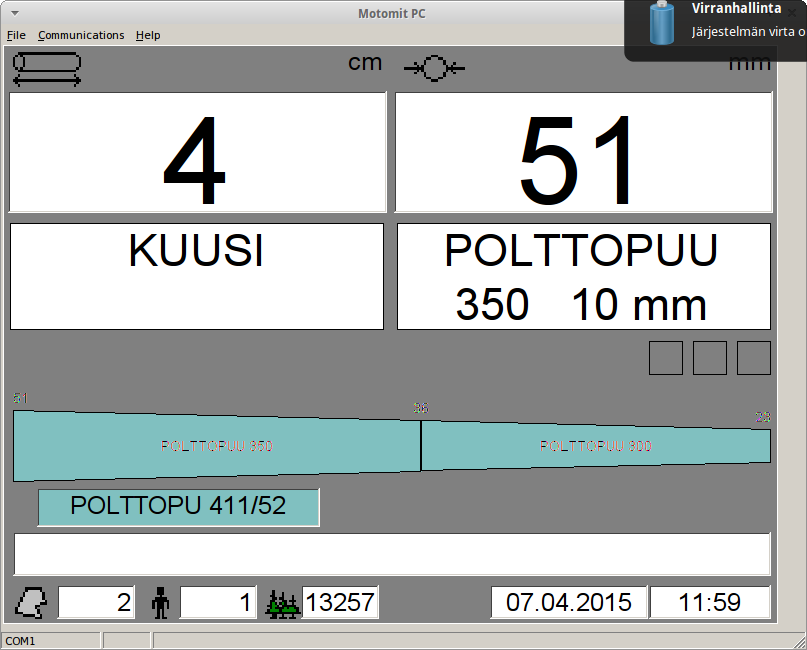
\includegraphics[width=1.00\hsize]{motomit_linux.png}
\caption{Motomit PC-ohjelmisto Winessä ajettuna.}
\end{figure}


\newpage

\chapter{Korvaava järjestelmä}
\label{ch:korvaava_jarjestelma}

Tämän työn aikana tehtyjen tutkimusten perusteella olen päätynyt esittämään yrittäjälle seuraavia vaihtoehtoja ajoneuvotietokoneen korvaamiseksi.

\section{Uusi ajoneuvotietokone}

Ehdotan ajoneuvotietokoneeksi Panasonic Toughbook CF-19 tietokonetta. Toughbook CF-19 on tabletiksi kääntyvä, täysvahvistettu kannettava joka on suunnitteltu ääriolosuhteisiin. CF-19 on suojattu niin, että se kestää pölyä, tärinää, iskuja ja -20 ja +60 °C välisen lämpötila-vaihtelun. CF-19 on varustettu Intel Core 2 Duo U7500 -prosessorilla, 4 Gb:n muistilla ja 10.4 \" näytöllä. Laite on IP54-suojattu kuten alkuperäinen ajoneuvotietokone ja se täyttää sähkömagneettisen yhteensopivuuden, tärinän, tiputuksen, vesi- ja pölytiiviyden, lämpötilankeston ja kosteudenkeston osalta Yhdysvaltain armeijan asettamat standardit. \cite{cf19}

Valitsin Toughbook CF-19 korvaajaksi, koska kääntyvän näytön takia sen saa n. 5 cm paksuksi, mikä mahdollistaa sen, että ko. kannettavalle voidaan toteuttaa helposti teline joko alkuperäiseen pidikkeeseen tai erillisenä kiinnityksenä. CF-19:sta löytyy lisäksi vakiona yksi RS-232 -sarjaportti, joka on luotettavuudeltaan parempi kuin USB-pohjaiset adapterit. Tällöin Motomit PC voidaan liittää sarjaporttiin ja Terman laittaa menemään USB-adapterin kautta tulevasta sarjaportista. Vaikka Panasonic Toughbook CF-19 on suhteellisen vanha (julkaistu v. 2007) \cite{cf19}, niin kyseistä mallia on hyvin saatavissa käytettyjen ja kunnostettujen tietokoneiden myyntiin erikoistuneista liikkeistä. Kosketusnäytön ansiosta erillistä hiirtä ei tarvita ja näppäimistöksi riittää ulkoinen näppäimistö.

\begin{figure}[H]
\centering
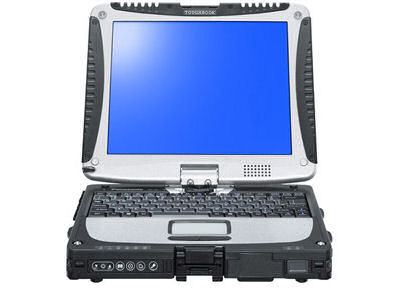
\includegraphics[width=0.50\hsize]{cf19.jpg}
\caption{Panasonic Toughbook CF-19.}
\end{figure}

\section{Uusi ajoneuvotietokone vanhaan kiinnikkeeseen}

Vaihtoehtona on myös suunnitella ja rakentaa vanhan kiinnikkeen kanssa yhteensopiva kotelo, johon asennetaan sopivan kokoinen näyttö, esim. RPI/2 -tietokone tai vastaava, sekä tarvittavat virtalähteet. RPIlle löytyy sekä Dosbox/rpix86 DOS-emulointiin, sekä ExaGearin avulla pitäisi pystyä ajamaan wineä. X86-tietokoneita löytyy myös riittävillä tehoilla pieninä mini-ITX -versioina.

Alkuperäinen kotelo on mitattu huollon yhteydessä, jotta uutta koteloa voisi harkita. Uusi kotelo antaa enemmän liikkumavaraa osien koolle ja sijoittelulle, mutta vaatii tarkempaa suunnitelua ja sovittelua. Kotelosta suunnitellaan 3D-malli, joka sitten voidaan 3D-tulostaa (tai tulostuttaa). Kotelon mitat on sen verran suuria, että osien suoratulostus ei taida olla kuluttajalaitteilla mahdollista ja täten 3D-mallia suunnitellessa se tulee ottaa huomioon. Myös pöly- ja kosteudenkesto tulee huomioida suunnittelussa ja toteutuksessa.

Vaihtoehtona on myös rakentaa valmiille kannettavalle yhteensopiva kiinnityslaite, jolloin vältytään mahdollisilta itse kasatun järjeseelmän kosteus- ja pölyongelmilta. Kiinnityslaitteen suunnittelu vaatii tiedon käytettävän tietokoneen mitoista, mutta totetus on samantapainen kuin uudella kotelolla, 3D-mallin suunnittelu ja tulostus/tilaus. Koska kotelon tulee olla varsinkin näytön takia riittävän suuri, voi olla helpointa tilata kotelo 3D-tulostuspalvelusta. Tulostuspalveluilta löytyy runsas joukko eri tulostusmateriaaleja joista voi valita kappaleeseen sopivimman, sekä tulostuspalveluiden käyttö mahdollistaa isompien 3d-kappaleiden tulostuksen, kuin yleisimmät harrastelijakäyttöön suunnatut 3d-tulostimet mahdollistavat. \cite{3d_shapeways} \cite{3d_ultimaker}

%Tulostaessa tulee huomioida. että pienemmissä 3D-tulostimissa käytetään pääsääntöisesti 2 eri muovityyppiä, ABS-muovia sekä PLA:ta. ABS (akryylinitriilibutadieenistyreeni) on muovina jäykkää, kestävää ja kevyttä, sekä edullista. Sitä käytetäänkin mm. autojen muoviosissa, sekä Lego-palikoissa. Tulostuksessa ABS-muovin haittapuolina on tulostuksen aikainen vääntyily (jota ehkäistään lämpölevyllä), sekä korkeahko sulamislämpötila. PLA (Polylaktidi) on uusiutuvista raaka-aineista tuotetuttu muovi. PLA on kovempaa kuin ABS, sekä se sulaa pienemmässä lämpötilassa. PLA on kuitenkin biohajoavaa, joten sen sopivuus motossa olevaan käyttöympäristöön ei ole taattua.


\section{Uusi ajoneuvotietokone vanhoihin kuoriin}

Toinen vaihtoehto on toteuttaa uusi tietokone Sunit Neron koteloon. Tämän vaihtoehdon etuna on se, että se olisi varmasti yhteensopiva alkuperäisen pidikkeen kanssa. Vaihtoehto vaatii tarkan mietinnän komponenttien valinnan ja kiinnityksen osalta, jotta toteutus saadaan kestämään varsinkin lämpötilavaihteluita ja tärinää. Alkuperäinen kotelointi tarjoaa IP54-luokiteltuna riittävän suojan pölyä ja vesiroiskeita vastaan.

Tässä vaihtoehdossa toteutus on vastaava kuin uusien kuorien tekemisessä, nyt vain sovitetaan vastaavat osat jo olemassa olevaan runkoon. Vanhan kotelon hyödyntämisessä on muutamia käytännön esteitä. Alkuperäistä konetta ei tulla ottamaan pois käytöstä, joten ainoaksi vaihtoehdoksi jää vastaavan koneen hankinta käytettynä. Koska kyseessä on kuitenkin jo 17 v vanha, erityiskäyttöön suunniteltu laite, niin vastaavan koneen/kuorien saatavuus on heikko ja hintapyynti voi olla kova suhteessa vastaavan kotelon uudelleentoteutukseen.



% \lipsum[1-5]

%http://www.adafruit.com/products/1287
%http://www.mini-box.com/M3-ATX-DC-DC-ATX-Automotive-Computer-car-PC-Power-Supply

% \section{Raspberry Pi 2}

% Raspberry Pi Foundation julkaisi helmikuussa 2015 uuden version suositusta yhden piirin Raspberry Pi -tietokoneestaan, Raspberry Pi 2:n. Raspberry Pi 2 sisältää järjestelmäpiirinä ARMv7-arkkitehtuuria käyttävän Broadcom BCM2836 -piirin sekä 1 Gb muistia. Raspberry Pi 2 on sovelluksesta riippuen 4-8 kertaa ensimmäisen Raspberry Pi:n käyttämää BCM2835 -piiriä nopeampi \cite{raspi2:perf}. Koska Raspberry Pi on saatavissa ominaisuuksiin nähden edulliseen n. 50€ hintaan, se antaa aihetta vähintäänkin harkita järjestelmän toteutusta RP2:n avulla.

% Fyysisesti toteutus olisi D53427RKE-pohjaisen ratkaisun kanssa yhtenevä, mutta tarvittavia osia olisi vain itse Raspberry Pi 2, microSD -kortti käyttöjärjestelmälle, 10,1" näyttöpaneeli sekä virtalähde. Virtalähteen ei tarvitse olla kovin tehokas, koska käytettävien osien tehonkulutus pudottaa osien vaatiman keskikulutuksen n. 10 Wattiin (Raspberry Pi 2: 4W, näyttöpaneeli n. 5W).

% Suuntaa antavasti hintaa Raspberry Pi 2-pohjaiselle ratkaisulle tulisi n. 50€ (Rpi2) + 20€ (32 Gb muistikortti) + 150€ (paneeli) + 30€ (virtalähde). Yhteensä siis n. 250€ + työt.

% ARM-arkkitehtuurista johtuen ohjelmistojen siirto tulee toteuttaa joko täysin emuloimalla esimerkiksi QEMU- tai Bohcs-emulaattorissa tai vaihtoehtoisesti käyttämällä esimerkiksi kaupallista Eltech Desktop x86 -binääritulkkainta. Näiden vaihtoehtojen toimivuutta ei kuitenkaan ole selvitetty tässä insinöörityössä ja ne vaatisivat lisäselvityksiä ja testauksia ennen mahdollista toteutusta.

% Raspberry Pi 2:ta ei ole ainakaan vielä julkisesti testattu EMC-määritysten osalta. Alkuperäinen Raspberry Pi on testattu EU:n asettamien määritysten mukaiseksi  \cite{raspi:emctesting}. EMC-vaatimusten täyttäminen on pakollista vasta valmiille, tuotantokäyttöön sellaisenaan tarkoitetuille tuotteille, mutta toteutuksessa kannattaa huomioida, että tulevan tietokoneen suojauksissa on otettu myös mahdolliset molempiin suuntiin kohdistuvat sähkömagneettiset häiriöt huomioon.

% \lipsum[1-5]


\newpage

\chapter{Yhteenveto}\

%% KORJAUSKOMMENTTI: Kolmas asia on työn tulokset. Minä en raportoisi siitä mitä metsäkoneelle ei tehty, vaan kertoisin vain mitä on tehty: valmis levykuva/asennuspaketti emulointiympäristöineen, testaus nauhoitetulla datalla, sopivan tietokoneen valinta ja kiinnityksen kuvaus. Se, että pakettia ei ole vielä asennettu (eikä ehkä asennetakaan) on asia, jonka esittely turhaan laskee työn arvoa. Työssähän on alussa todettu että kone on aktiivikäytössä, joten voit vaikka todeta että asennusvalmius on sitten kun tulee seuraavan ison huoltoseisokin aika tms....

Insinöörityön tavoitteena oli selvittää työn kohteena olevan 17 vuotta vanhan hakkuukoneen alkuperäisen ajoneuvotietokoneen liitännät ja ohjelmistot sekä tutkia mahdolliset vaihtoehdot korvata vanha, käyttöikänsä loppupäässä oleva alkuperäinen ajoneuvotietokone uudemmalla, hakkuukoneen järjestelmien kanssa yhteensopivalla vaihtoehdolla. Alkuperäinen tarkoitus oli tutkia vaihtoehdot, sekä toteuttaa käyttökuntoon asti korvaava tietokone.

%Projektin aikana kuitenkin alkuperäisen tietokoneen huollon jälkeisen toiminnan parantuminen, sekä taloustilanteen huonontumisen takia päädyttiin jättämään varsinainen toteutus varavaihtoehdoksi ja keskittymään totetuksen esivalmisteluun.

Alkuperäistä ajoneuvotietokonetta tutkimalla sekä mahdollisia vaihtoehtoja punnitsemalla päädyttiin testaamaan alkuperäisten ohjelmistojen toimivuutta yhteensopivuusrajapintojen kautta tavallisessa, useamman vuoden vanhassa Linux-käyttöjärjestelmällä varustetussa kannettavassa tietokoneessa. Testaamalla selvisi, että käytettävät alkuperäiset ohjelmistot toimivat USB-sarjaporttiadapterin ja Linuxin kautta suoritettuina. Tästä voidaan päätellä että alkuperäinen Sunit Nero-ajoneuvotietokone on helpostikin korvattavissa uudemmalla olosuhteita kestävällä ajoneuvotietokoneella tai kannettavalla.

Vaatimuksina uudelle tietokoneelle on lähinnä tarvittava olosuhteiden kesto sekä tarvittavat liittimet. Hakkuukoneen järjestelmät vaativat kaksi sarjaporttiliitäntää, joilla kommunikointi hakkuukoneen ja ajoneuvotietokoneen välillä tapahtuu. Hakkuukoneen sähköjärjestelmä on 24V, mikä tulee ottaa huomioon tietokoneen sähkönsyöttöä pohdittaessa.

Työssä saatiin totetutettua ajoneuvokoneen korvaavan tietokoneen levykuva, sekä suoravaiivaiset asennusohjeet uudelleenasennukseen. Levykuvan ja tavallisen kannettavan avulla saatiin testattua ohjelmistojen toimivuus ajoneuvotietokoneen kanssa. Korvaavaksi tietokoneeksi, sekä sen kiinnittämiseksi metsäkoneeseen on tehty selvitykset. Koska alkuperäinen metsäkone ajoneuvotietokoneineen on aktiivikäytössä ja metsässä suurimman osan ajasta, pystytään uusi ajoneuvotietokone saattamaan asennusvalmiiksi metsäkoneen seuraavaan isompaan huoltoon mennessä.


Suurimmat haasteet insinöörityössä liittyivät pääsyyn työn kohteena olevalle hakkuukoneelle. Hakkuukone oli aktiivisessa käytössä Oriveden metsissä koko insinöörityön ajan ja vierailut koneelle saatiin lopulta järjestettyä alkuperäisen ajoneuvotietokoneen huoltojen yhteydessä. Hakkuukoneen kommunikointi ajoneuvotietokoneen kanssa osoittautui kuitenkin suhteellisen yksinkertaiseksi standardinmukaiseksi RS-232 sarjamuotoiseksi liikenteeksi.


%Alkuperäinen suunnitelma valmiista ajoneuvotietokoneen korvaajasta jäi saavuttamatta, mutta projekti on saatu pisteeseen, josta on helppo jatkaa toteutukseen. Ohjelmistoista on tehty valmiit levykuvat käytettäville arkkitehtuureille, sekä tarvittavat osat on mietitty ja alustavasti suunniteltu.




%\lipsum[12-14]

% Parhaana vaihtoehtona pidän tällä hetkellä ajoneuvotietokoneen korvaamista Panasonic Toughbook CF-19 tietokoneella. Myös Raspberry Pi 2-pohjainen ratkaisu on harkitsemisen arvoinen.

% Suurimmat haasteet insinöörityössä liittyivät pääsyyn työn kohteena olevalle hakkuukoneelle. Hakkuukone oli aktiivisessa käytössä Oriveden metsissä koko insinöörityön ajan ja vierailut koneelle saatiin lopulta järjestettyä alkuperäisen ajoneuvotietokoneen huoltojen yhteydessä. Hakkuukoneen kommunikointi ajoneuvotietokoneen kanssa osoittautui kuitenkin yksinkertaiseksi, joten järjestyneet käyntikerrat riittivät hyvin selvittämään alkuperäisen järjestelmän toimintaa sekä testaamaan mahdollisessa uudessa tietokoneessa käytettäviä ratkaisuja.

% %Muita haasteita työn toteutukselle toi hektinen arki. Tyttäreni syntyi joulukuussa vaikean raskauden päätteeksi ja mukana menossa on myös neljävuotias esikoinen. Täysipäiväisesti töitä tekevänä isänä en koe valitettavasti pystyneeni täysin antamaan insinöörityölle sen ansaitsemaa panostusta. Aion kuitenkin hyödyntää tekemääni työtä toteuttamalla uuden ajoneuvotietokoneen myös käytännössä.

% Insinöörityössä saavutettiin asetetut tavoitteet uuden tietokoneen vaatimusten ja toteutusvaihtoehtojen selvittämisestä. Tarkoitus on, että hakkuukoneeseen hankitaan vielä tämän vuoden aikana edellä mainitun suunnitelman mukaisesti uusi ajoneuvotietokone, joka voidaan ottaa käyttöön alkuperäisen ajoneuvotietokoneen hajotessa seuraavan kerran.

%Lopuksi haluaisin kiittää rakasta vaimoani Jennikaa kannustuksesta ja oikolukuavusta, poikaani Tuukkaa toimimisesta apulaisena alkuperäisen koneen huollon ja tutkimisen yhteydessä sekä hakkuukoneen omistajaa Arto Saalia, joka oli suureksi avuksi kaikissa käytännön järjestelyissä.\newline


% \begin{figure}[H]
% \centering
% 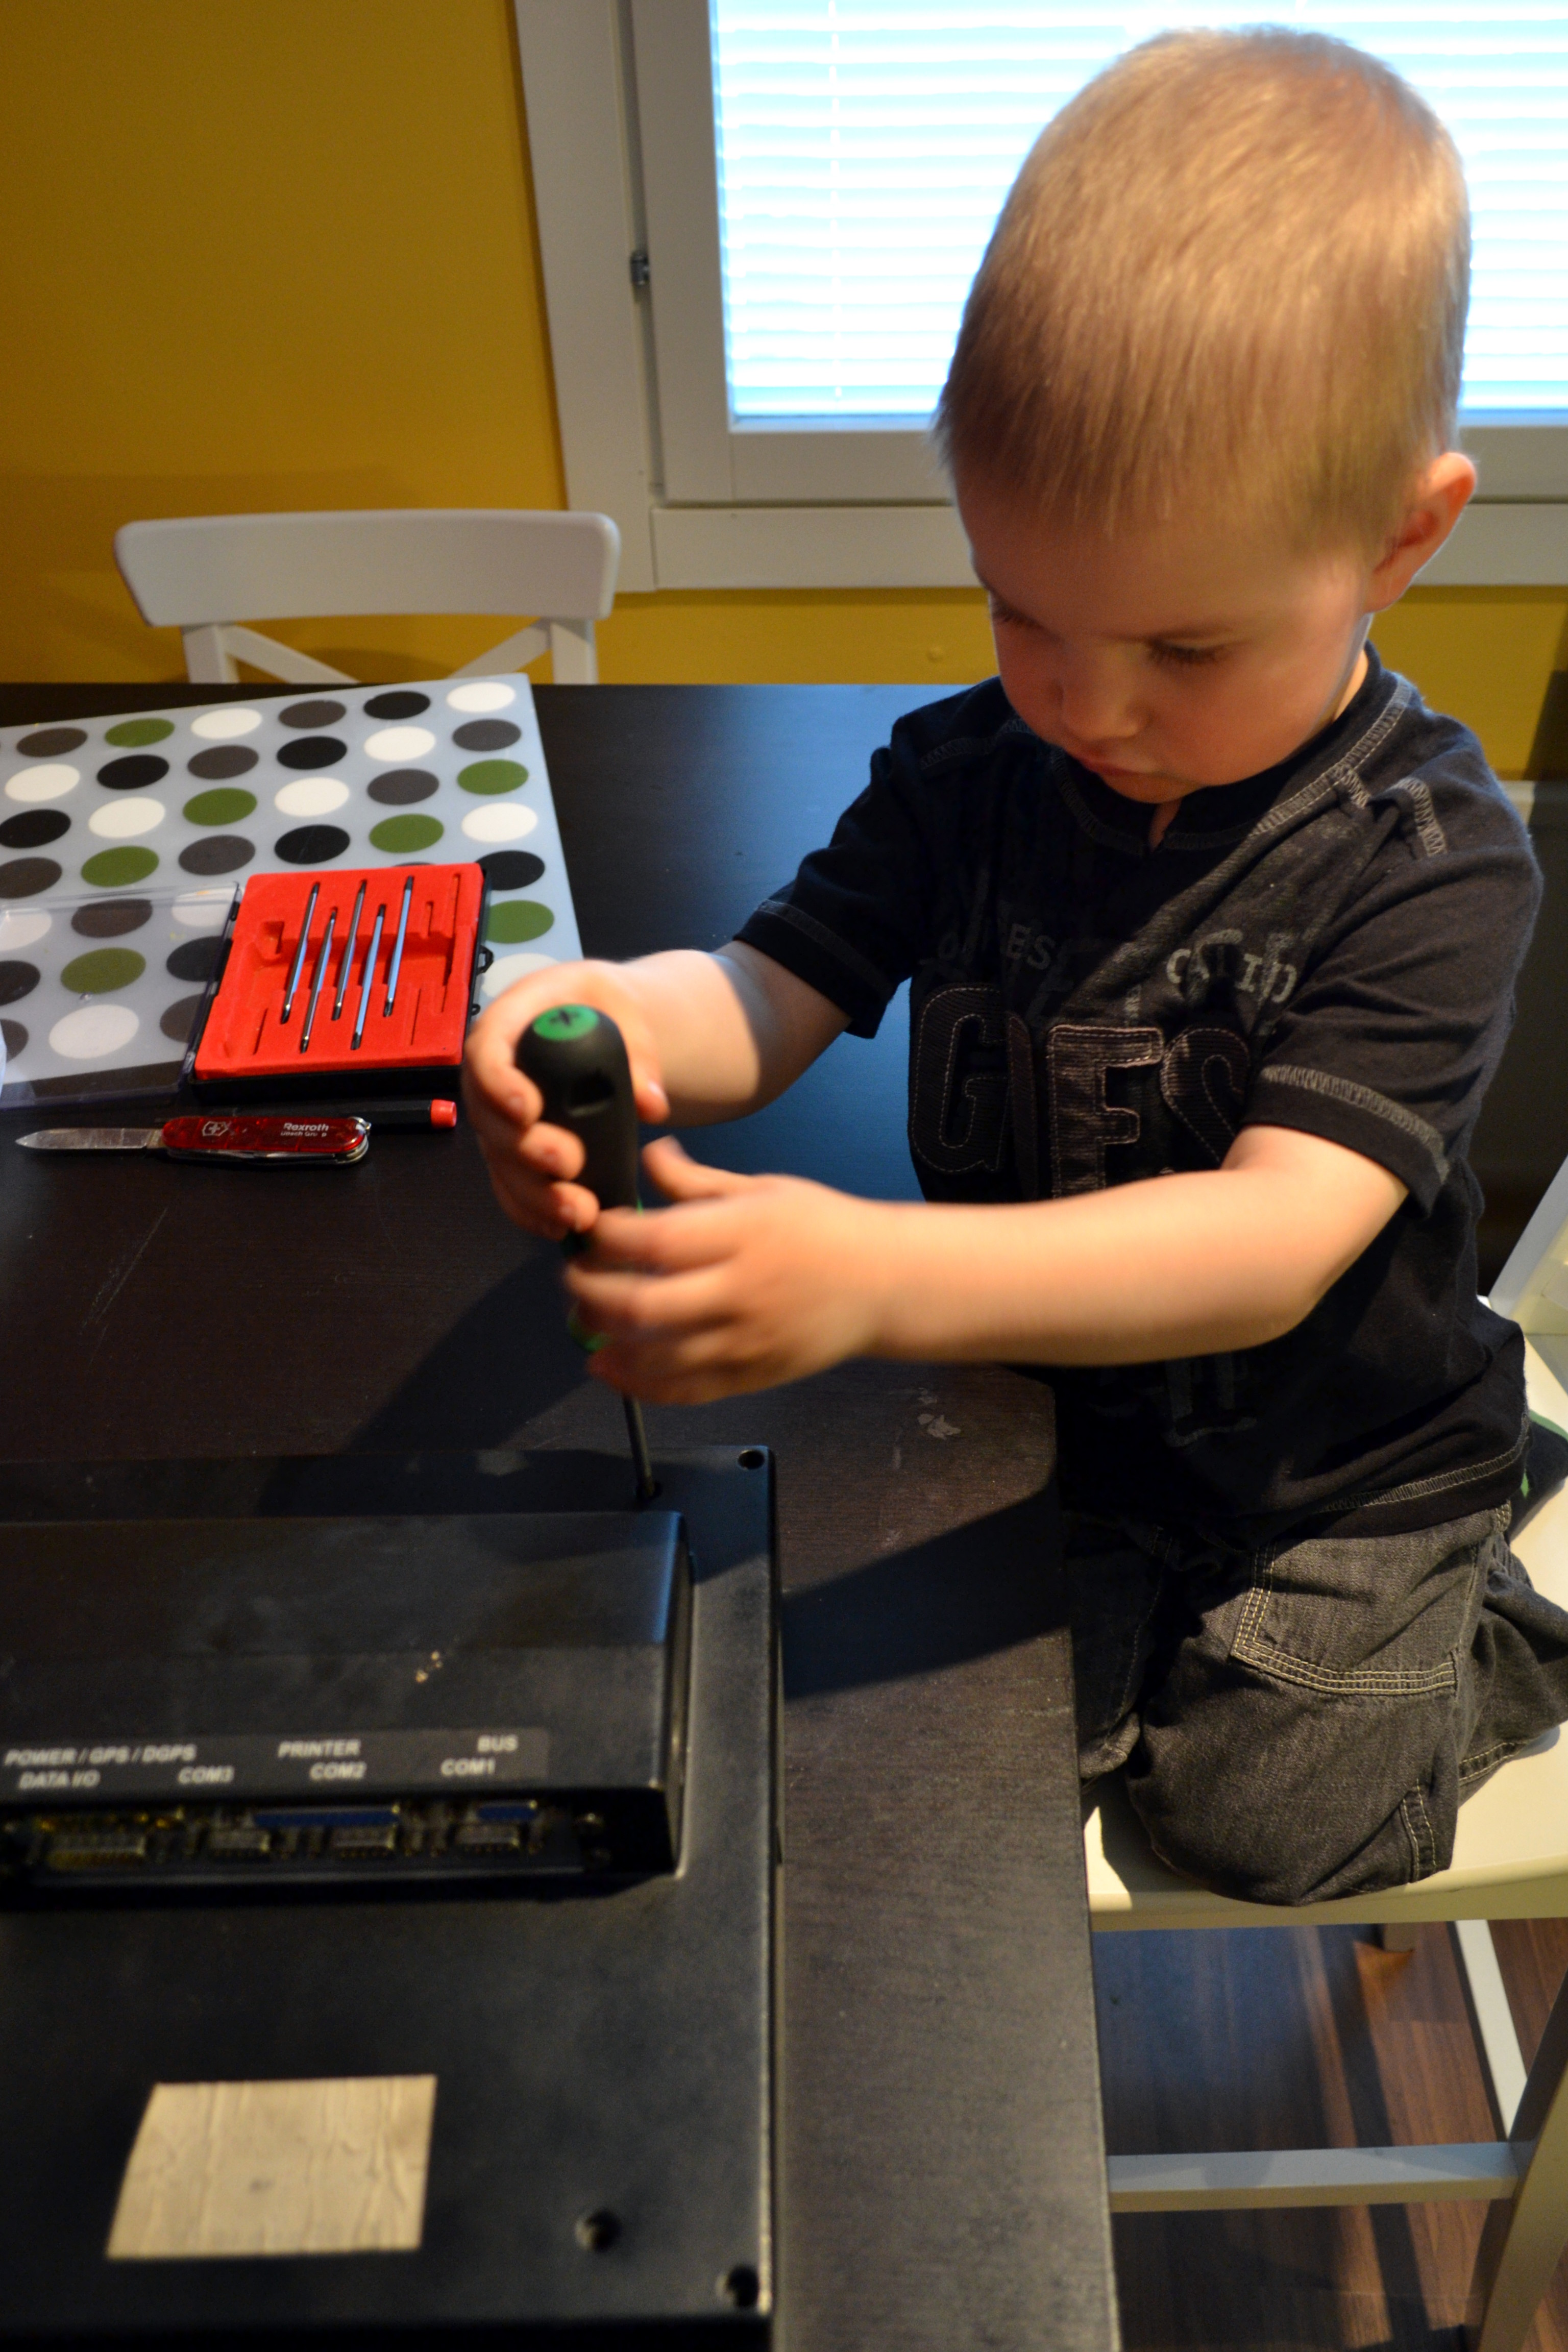
\includegraphics[width=0.80\textwidth]{tuukka_auttaa.jpg}
% \caption{Tuukka Haapaniemi valmistelemassa ajoneuvotietokoneen huoltoa}
% \end{figure}

\newpage

%----------------------------------------------------------------------------------------
%   BIBLIOGRAPHY
%----------------------------------------------------------------------------------------

\IfLanguageName{finnish}{\bibliographystyle{vancouver_fi}}{\bibliographystyle{vancouver}}
%line space
%\singlespacing %removed otherwise the appendix are also single space
\begin{flushleft}
\begin{singlespacing}
\bibliography{motonkone_biblio}
\end{singlespacing}
\end{flushleft}

%for conting the pages
\label{LastPage}%~

%\end{document}
